\documentclass[12pt,a4paper]{article}
\usepackage{hyperref} 
\usepackage{xcolor}
\usepackage{float}
\usepackage{amsmath}
\usepackage{booktabs}
\usepackage{graphicx}
\usepackage{csquotes}
\usepackage{subcaption}



\usepackage{graphicx} % Required for inserting images
\usepackage[left=1.4cm, right=1.4cm, top=1.9cm, bottom=1.9cm]{geometry}



\title{\Huge \textbf{Data Mining \\ Project Report}} 

\author{ \Large{Aliprandi Francesco} \\ \Large{Liuzzi Francesco Paolo} \\ \Large{Simonetti Francesco}}
\date{\large{A.Y. 2024/2025}}


\begin{document}

\begin{figure}
    \centering
    
\includegraphics[width=0.5\linewidth]{images/unipi.png} 
\end{figure}

\maketitle

\newpage

\section*{Introduction}
This report describes all the procedures and methodologies adopted to perform data analysis and mining on a dataset consisting of detailed information about professional cycling races. The analysis focuses on exploring various techniques, including understanding the data, data transformation, clustering, prediction, and AI explanation, to gain insights into cyclist performance over the years.\\

\noindent The report is organized as follows: Section 1 focuses on data understanding, including all the analyses necessary to comprehend the dataset. Section 2 details the data cleaning process, outlining all the interventions to refine the dataset. Section 3 addresses the feature engineering for clustering, providing explanations of the features created to tackle the clustering task. 
Section 4 discusses outlier detection performed before clustering and includes a thorough analysis of the clustering algorithms used. Section 5 presents the classification task, covering feature engineering, imbalance analysis, an exploration of the task's inherent complexities, and a comparison of all models tried. Finally, Section 6 delves into explainable AI, analyzing the decisions made by the best-performing classification model.

\noindent The project notebooks with a comprehensive and more detailed analysis can be reached at: \url{https://github.com/effepielle/dm_project24_group_0}

\section{Data Understanding}

The task involved exploring the two assigned datasets: \texttt{cyclists.csv}, containing information about the cyclists, and \texttt{races.csv}, which includes race results and race-related data over the years. This provided an overall understanding of the data, which was useful for subsequent analysis and modeling tasks.

% -------------- cyclists dataset ------------------
\subsection{Cyclists Dataset}
\textbf{Dataset Overview and Key Insights}\\
The dataset consists of $6'134$ rows, each representing a specific cyclist. Each cyclist is identified by a unique \textit{\_url} and described by the following features: \textit{name}, \textit{birth\_year}, \textit{weight}, \textit{height}, and \textit{nationality}. The cyclists in the dataset have birth years ranging from 1933 to 2004. Based on the distribution, 75\% of the cyclists were born from 1962 onward, while only 25\% were born before 1962 (first quartile), indicating a much higher representation of cyclists born in more recent decades. \\
The \textit{height} and \textit{weight} of cyclists follow approximately a bell-shaped distribution. In particular, most cyclists have a height centered around 180 cm and a weight of around 70 kg. This suggests that cyclists tend to have a “standard” physique, with height and weight values centered around those values. \\
We can state that 86.50\% of cyclists are from Europe, and in particular, 57\% of the dataset consists of cyclists from only 4 European nations: Italy (the country with the most cyclists), Spain, Belgium, and France.\\
In terms of \textbf{feature correlations}, the only notable relationship observed is between \textit{height} and \textit{weight}, which aligns with expectations that taller cyclists generally weigh more.\\

\noindent
\textbf{Null Values and Outliers}\\  
The features \textit{\_url} and \textit{name} have 0 null values, \textit{nationality} has only 1 null value, \textit{birth\_year} has 13 null values, while \textit{weight} and \textit{height} have many null values, with half of the values missing for both. The null values are observable in \autoref{fig:null_values}. Excluding \textit{birth\_year}, all other numerical features exhibit outliers that follow either a symmetric distribution or are slightly skewed, as shown in the box plots presented in the notebook.\\

\noindent
\textbf{Consistency}\\
There are duplicate cyclist names, but no duplicate URLs. As we show in the notebook, usually the same name is associated with different cyclists which can be discriminated by a different URL and other feature values, if available.\\

\begin{figure}[H]
    \centering
    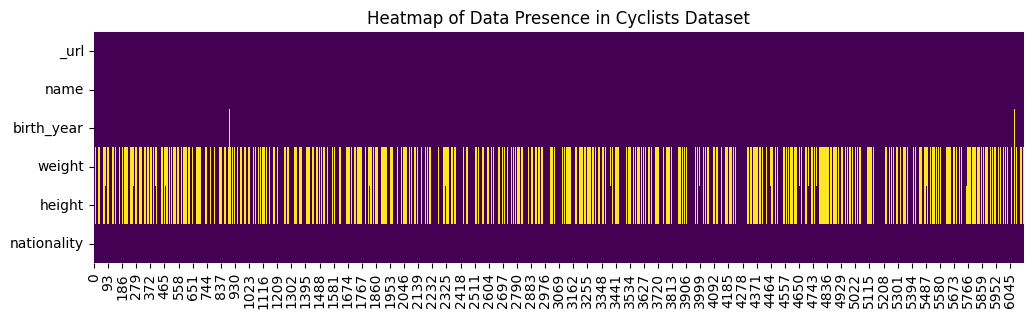
\includegraphics[width=0.7\linewidth]{images//DU/null_values.png}
    \caption{\small Null value heat-map in cyclists dataset}
    \label{fig:null_values}
\end{figure}

% -------------- Races dataset ------------------

\subsection{Races Dataset}

The dataset contains over $589'865$ rows, organized by race and stage. Each race, such as the "Giro d'Italia", is represented by multiple stages, and each stage is identified by a unique \textit{\_url}. The dataset includes several rows for each cyclist participating in the same stage, leading to the repetition of stage-related information. Additional features capture cyclist-specific details, including their identity, age, and team affiliation. 

\subsubsection{Feature overview}


\noindent \textbf{\_url}: this categorical alphanumeric column contains the unique URL identifier for each race stage and is repeated for every cyclist participating in that stage. \\

\noindent \textbf{name}:
This categorical alphanumeric column represents the race name for each stage, with 27 unique race names in the dataset. Variations in names arise from minor differences in spelling, accents, or naming conventions over time. For instance, \enquote{san-sebastian} corresponds to names like \enquote{Clasica Ciclista San Sebastian}, \enquote{Clásica Ciclista San Sebastián}, and \enquote{Clásica San Sebastián}, all referring to the same race.\\ 

\noindent \textbf{points}: 
This numerical attribute represents points assigned by the race, which can be the same for multiple cyclists. There are 4 stages with null values, resulting in a total of 477 null rows, but there are no illegal values (such as negative numbers, extreme outliers, or inconsistent values for the same stage). The points range from 50 to 150, with 50 being the most frequent value. The average is 89, and the median is 80.
On average, we can notice that the average point values are decreasing over the years.\\ 

\noindent \textbf{uci\_points}: This feature is similar to the previous one, but the points here are the official ones assigned by the UCI organ. There are $3'862$ stages with missing values, totaling $338'779$ rows in the dataset. The values range from 6 to 800, with the most frequent values being 100, 6, and 60. The mean is 82, and the median is 60.\\

\noindent \textbf{length}: this feature represents the total stage length in meters, with values ranging from 1 km to 338 km and a mean of 166 km. There are no null or inconsistent values in this feature, and the distribution exhibits two peaks: one for very short races and another for longer races. \\

\noindent \textbf{climb\_total}: this feature represents the total elevation gain of the stage in meters, with values ranging from 2 m to $6'974$ m and a mean of $2'375$ m. There are $2'214$ stages with null values, totaling $147'045$ rows, but no inconsistent values. The distribution shows two peaks: one for stages with minimal elevation gain and another for stages with higher elevation gains. This reinforces the idea mentioned earlier: there are primarily two types of races, shorter ones and longer ones.\\

\noindent \textbf{profile}: this categorical feature represents the race profile, with increasing difficulty levels ranging from 1 to 5, corresponding to: flat, hilly, mountainous, high mountains, and high mountains with an uphill finish. There are $2'408$ stages with null values, totaling $148'194$ rows, but no inconsistent values. The most represented classes are the first and second, with the latter being the median. \\

\noindent \textbf{startlist\_quality}: this numerical feature represents the strength of participants in the race. Higher values indicate stronger cyclists, while lower values correspond to weaker cyclists. The feature contains no null or inconsistent values. Values range from 115 to $2'047$, with a mean of 989. The distribution is bell-shaped, with some peaks for higher start list quality values. Analyzing the average start list quality across stages over the years shows an increasing trend, except for 2020, when the COVID-19 pandemic led to fewer races with lower start list quality. \\

\noindent \textbf{average\_temperature}: this feature represents the average temperature recorded for a particular stage. However, since 97\% of the stages have null values for this feature, no further investigation was conducted.\\

\noindent \textbf{date}: This feature includes both the stage's starting date and the completion time for each cyclist. For analysis purposes, we split it into \textit{start\_date} and \textit{duration}. Stage dates range from 1970-02-28 to 2023-07-29, with an average year of 2001. As reported in \autoref{fig:start_date} number of stages generally increased until the late 1980s, then stabilized with slight fluctuations through the 1990s and 2000s. A notable drop occurred in 2020 due to the COVID-19 pandemic, though not all races were canceled, as reported by \href{https://www.procyclingstats.com/statistics.php}{ProCyclingStats}. \\ The \textit{duration} column mirrors the values in the \textit{delta} column, so correctness analysis focuses on the latter. The distribution appears bell-shaped with two peaks, reflecting both short races with low durations and longer races with higher durations. Longer races dominate, with an average duration of 4 hours and 24 minutes. There are no null values in both features.\\

\begin{figure}[H]
    \centering
    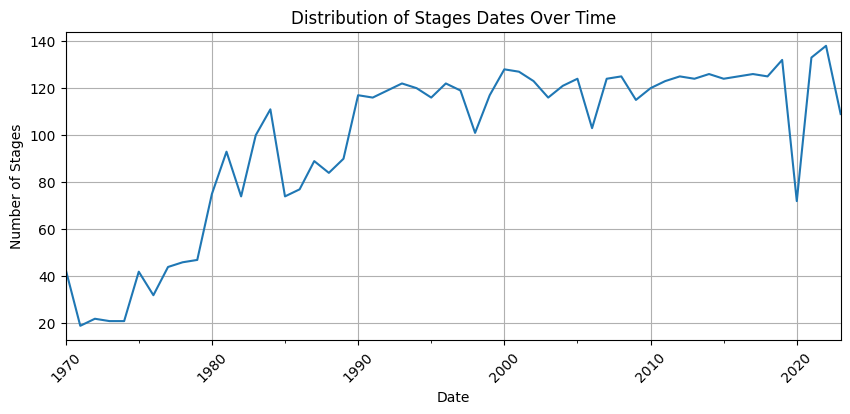
\includegraphics[width=0.5\linewidth]{images//DU/start_date_plot.png}
    \caption{\small Stages frequency per year plot}
    \label{fig:start_date}
\end{figure}


\noindent \textbf{position}: it ranges from zero to the total number of participants minus one, with all values being valid and following a monotonically increasing order.\\

\noindent \textbf{cyclist}: it contains the unique identifiers for cyclists. We noticed 249 duplicate entries within the same stages, which will be addressed during the \autoref{sec: data_cleaning} phase. No null values are present.\\

\noindent \textbf{cyclist\_age}: this feature represents the age of cyclists in a specific stage. It includes 113 null entries, with ages ranging from 13 to 56 years and an overall average of 28 years. To avoid skewing caused by cyclists appearing in multiple stages, we analyzed the average cyclist age per stage. The average age ranges from a minimum of 23 to a maximum of 31 years. When visualizing the average age across stages (averaging over all stages in a given year), we observe an increasing trend in the average age over time.\\

\noindent \textbf{is\_tarmac}: this binary feature indicates whether the stage surface is tarmac or not. There are no missing values, and 19\% of the feature values are false for individual stages, with the same value being applied to all instances of a given stage. \\

\noindent \textbf{is\_cobbled}: this binary feature indicates whether the stage surface is tarmac or not. All values are set to false, so the feature is unusable. \\

\noindent \textbf{is\_gravel}: this binary feature indicates whether the stage surface is gravel or not. All values are set to false, so the feature is unusable.\\

\noindent \textbf{cyclist\_team}: this alphanumeric feature represents the cyclist's team. A cyclist may have competed with different teams throughout their career.\\

\noindent \textbf{delta}: this numeric column represents the time difference between the current cyclist and the first-place finisher. We observed that it perfectly matches the duration column and contains $3'239$ non-increasing values with also some wrong negative values. As a result, we decided not to use this feature and instead focus the analysis on stage winners.\\

\noindent
\textbf{Null Values}\\
As for cycling datasets, we reported the heat map of null values in \autoref{fig:raes_heatmap}, to better visualize null values in the dataset.

\begin{figure}[H]
    \centering
    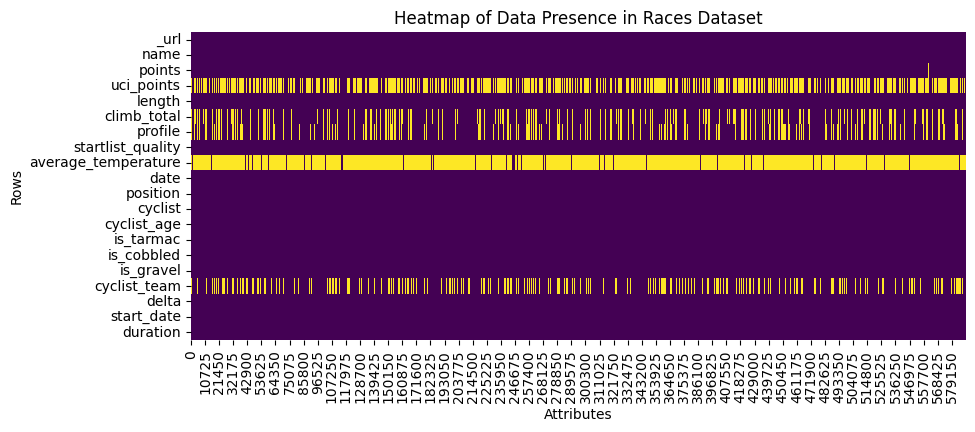
\includegraphics[width=0.6\linewidth]{images//DU/heatmap_races.png}
    \caption{\small Races null values heat-map}
    \label{fig:raes_heatmap}
\end{figure}


\noindent
\textbf{Correlations}\\
The only features with a slightly higher correlation are \textit{profile} and \textit{climb\_total} as races with a higher profile (such as mountainous or high-mountainous races) typically involve a greater number of kilometers climbed.\\

\begin{center}
    \begin{figure}[H]
    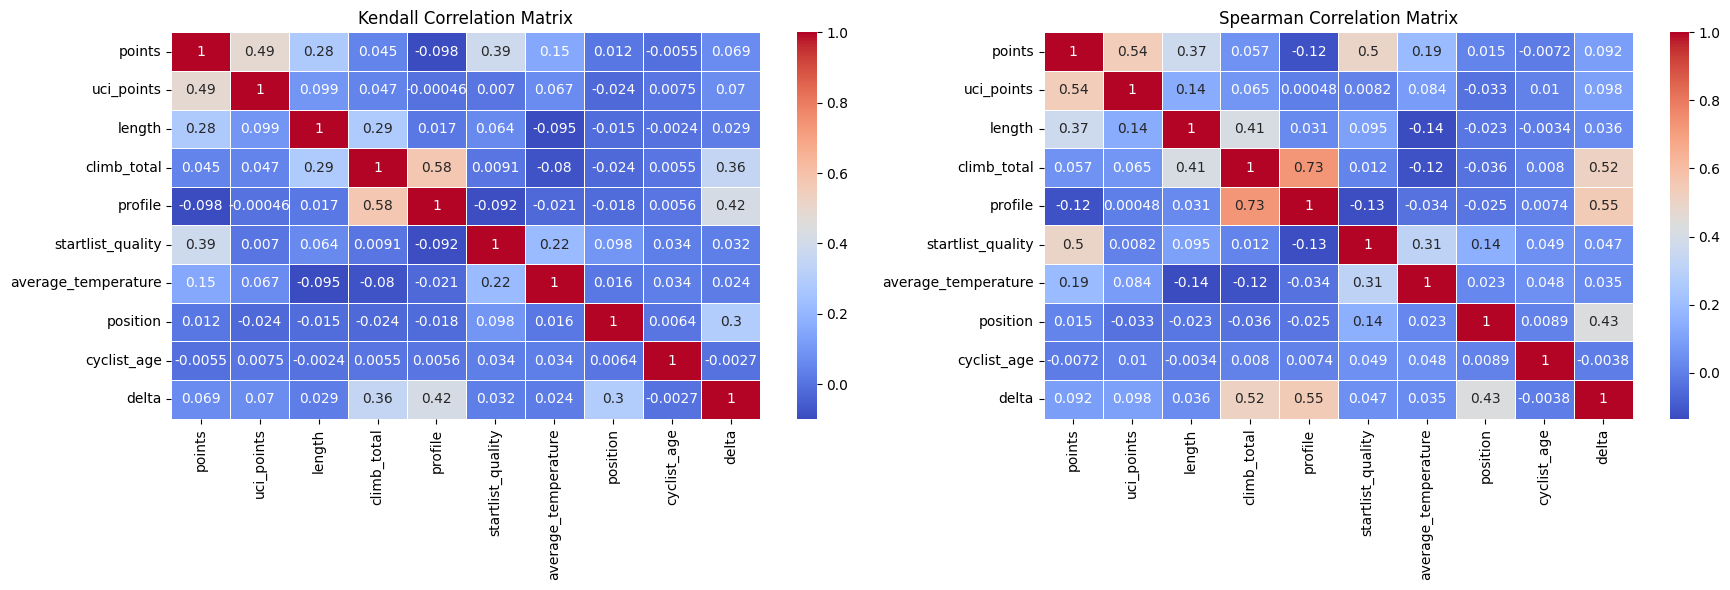
\includegraphics[width=0.9\textwidth]{images/DU/races_corr.png}
    \caption{Correlation between numerical features in races dataset}
    \end{figure}
\end{center}

\vspace{-1.2cm}
\noindent
\textbf{Consistency and issues}\\
A check was conducted to verify whether all features, whose values are replicated across all rows for a given stage were consistent in their copies. For example, the length should remain the same for all copies within a specific stage and all features were found to be consistent. \\
The main issues identified in the dataset are the following:

\begin{itemize}
    \item \textbf{Race terrain features:} The categorical boolean features \textit{is\_cobbled} and \textit{is\_gravel} are always false, unlike \textit{is\_tarmac}. As a result, whenever \textit{is\_tarmac} is false, the other two features do not provide any useful information.
    \item \textbf{Incorrect delta values:} This value represents the time difference between a cyclist and the race winner. However, in many races this value is negative, making it meaningless. We also attempted to calculate these values by checking the start and finish times of the races, but we found that they were consistent with the reported delta values. We observed several cases where cyclists in position $m$ had a total time lower than cyclists in position $n$, where $m > n$. This is logically impossible and further confirms the inconsistencies in the data.
    \item \textbf{Duplicated cyclists:} There are stages where a cyclist appears multiple times in different positions.
\end{itemize}


% -------------- Both dataset ------------------


\subsection{Races and Cyclists dataset}
Comparing the two datasets, it was confirmed that every cyclist who has competed is included in the cyclist's dataset. Instead, the opposite was found: there are about ten cyclists who have never participated in any race (according to our data).\\

\noindent
In the notebook \texttt{'TASK\_1/data\_understanding.ipynb'}, one can find all the details for each feature of both datasets, including distributions and box plots.\\








\section{Data Cleaning}
\label{sec: data_cleaning}

\subsection{Cyclist dataset}

\textbf{Birth Date}:
The missing birth dates of the cyclists were assigned as follows: the average debut age was calculated, and using the cyclist's first race as a reference, this average age was subtracted from the date of the race to approximate birth date. This approach was used because there were not many null values for this feature.\\

\noindent
\textbf{Nationality}:
Regarding nationality, it was imputed by manually checking online, as there was only one missing value. \\

\noindent
\textbf{Height and Weight}:
Height and weight data are missing for approximately half of the entries. Given the correlation between these features, the initial plan was to estimate one value from the other when only one was missing, and then handle any remaining missing values either through approximation or by discarding rows if their number was minimal. However, as shown in \autoref{fig:null_values}, height and weight are often missing simultaneously, making it infeasible to reliably impute these values for a significant portion of the dataset.

\subsection{Races dataset}
All rows that represent duplicate cyclists for the same stage URL were removed. We dropped both duplicates since we didn’t know which one was the correct one.\\

\noindent
\textbf{points}:
Only four over more than five thousand stages do not have point information. So we decided to impute missing values using a segmentation approach: we imputed the median value of that particular stage over the years. \\

\noindent
\textbf{uci\_points}:
As they have a lot of missing values and we have points information, we decided to drop this column.\\

\noindent
\textbf{length and climb\_total normalization:} both features are normalized to avoid excessively large values. Length is now represented in hundreds of kilometers, while climb total is measured in kilometers.\\

\noindent
\textbf{climb\_total and profile cleaning:}
Given that the two features contain a significant number of null values but they are critical for evaluating stage complexity, we initially considered dropping rows with null values. However, since this cleaning step would result in the removal of more than $140'000$ rows and more than $2'000$ stages, we decided to postpone this step to preserve stage information that could be valuable for feature engineering of the cyclist's dataset. \\

\noindent
\textbf{average\_temperature:}
Since we have very few known values, we decided to drop the column.\\

\noindent
\textbf{is\_cobbled and is\_gravel:}
Since all the values are set to "False" so they are not informative, we decided to drop the columns.\\

\noindent
\textbf{delta:}
Since the delta column contains many incorrect values (as explained in data understanding), the column is not useful for our analysis, so we decided to drop it.\\

\noindent
\textbf{Note:} Due to the reasons outlined for the features \textit{climb\_total} and \textit{profile}, some rows will still contain null values after this initial phase of data cleaning.

\section{Feature Engineering for Clustering}
\label{sec:feat_eng}
In this phase, we focused on creating features specifically for the cyclist dataset, as the subsequent clustering step was performed exclusively on this data. However, the race dataset was also essential for calculating these features, as the new cyclist features were derived from their career performance. Initially, features were also created specifically for the race dataset during an exploratory phase, but these were ultimately not used since the decision to cluster only on the cyclist dataset was made later.
To focus the analysis on professional cyclists, we selected those with more than 20 races to date. This filtering was done before the feature engineering step to not alter the distributions of the engineered features.

\subsection{Engineered Features Overview}

\noindent
\textbf{cyclist\_experience:} counts how many stages the cyclist participates in as an overall experience.\\

\noindent
\textbf{cyclist\_experience\_points:} It represents the total points accumulated by each cyclist in the races they participated in (not weighted by position). \\

\noindent
\textbf{cyclist\_win:}
count how many stages are won by each cyclist.\\

\noindent
\textbf{cyclist\_win\_ratio:} compute the ratio between stages won and stages in which the cyclist participated. \\

\noindent
\textbf{avg\_position:} it is the average position considering all the races the cyclist has participated in.\\

\noindent
\textbf{avg\_relative\_position:} This feature represents the average placement of a cyclist throughout their career, with each position normalized according to the number of participants in each race.\\

\noindent
\textbf{min\_relative\_position:} it is the best (minimum) relative position achieved by a cyclist.\\

\noindent
\textbf{relative\_position\_std:} this feature highlights a cyclist's performance consistency: a low standard deviation indicates steady results, while a high standard deviation reflects variability influenced by factors like race difficulty or participant numbers or weather conditions, etc.\\

\noindent
\textbf{best\_position:} it is the best (minimum) position achieved by a cyclist.\\

\noindent
\textbf{position\_std:} It's like \textit{relative\_position\_std} but the position is not normalized by the number of cyclists.\\

\noindent
\textbf{mean\_last\_20\_positions:} This feature represents the average position achieved in the 20 worst performances of a cyclist.\\

\noindent
\textbf{mean\_last\_20\_positions\_1:} This feature is similar to the previous one, but the worst placements are selected based on relative ranking rather than solely considering absolute position when identifying the 20 worst performances. \\

\noindent
\textbf{avg\_position\_vs\_startlist}: the average relative position achieved by a cyclist, normalized by the start list quality to account for race difficulty.\\

\noindent
\textbf{performance\_entropy:} It's a performance variability metric. It measures the consistency of a cyclist's performance across races. Lower values indicate consistent results, while higher values reflect more fluctuating performance, similar to position standard deviation.\\

\noindent
\textbf{weighted\_podiums:} 
The value of the feature is calculated as follows:
\[
\text{Weighted Podium}_{j} =  \frac{1}{T_j}  \sum_{r=1}^{R} \left( w_i \cdot point_{r} \cdot N_r \right)
\]

\noindent
with \( r \) representing a specific race, ranging from 1 to \( R \), which is the total number of races. The variable \( w_i \) denotes the weight assigned to a cyclist's position ($w_1$ for first place, $w_2$ for second place, $w_3$ for third place, 0 otherwise). The points awarded for a race \( r \) are represented as \( point_r \). \( N_r \) is the total number of cyclists participating in race \( r \), while \( T_j \) indicates the total number of races completed by cyclist \( j \).\\


\noindent
\textbf{career\_level:} 
This feature represents the level of a cyclist by summing all the placements achieved in their career, weighted by the points of the races and considering the placements reached in their career, taking into account the points of the races they participated in and the number of cyclists in those races:
\[
\text{Career Level}_j = \sum_{r=1}^{R_j} \frac{(\text{N}_r - \text{pos}_{j,r}) \cdot \text{points}_r}{\text{N}_r}
\]

\noindent
\( r \) represents a specific race, ranging from 1 to \( R \) (the total number of races). The variable \(\text{pos}_{j,r}\) indicates the position of cyclist \( j \) in race \( r \). The points awarded for race \( r \) are represented as \(\text{points}_r\), and \( N_r \) refers to the total number of cyclists participating in race \( r \).\\

\noindent
\textbf{mean\_sq:} it represents the average start list quality of all the races the cyclist participated in. This feature represents somehow the "relevance" but also "the difficulty" on average of the stages in which a cyclist participated. \\

\noindent
\textbf{top\_cyclists:} this feature is calculated by dividing cyclists into ranked segments based on the ordered values of the \textit{career\_level} feature, such as top 10, top 20, and so on.\\

\noindent
\textbf{top\_experience:} it is calculated by dividing cyclists into ranked segments based on the ordered values of the \textit{cyclist\_experience} feature, such as top 10, top 20, and so on, to somehow categorize cyclists based on their experience. \\


\begin{figure}[H]
\centering
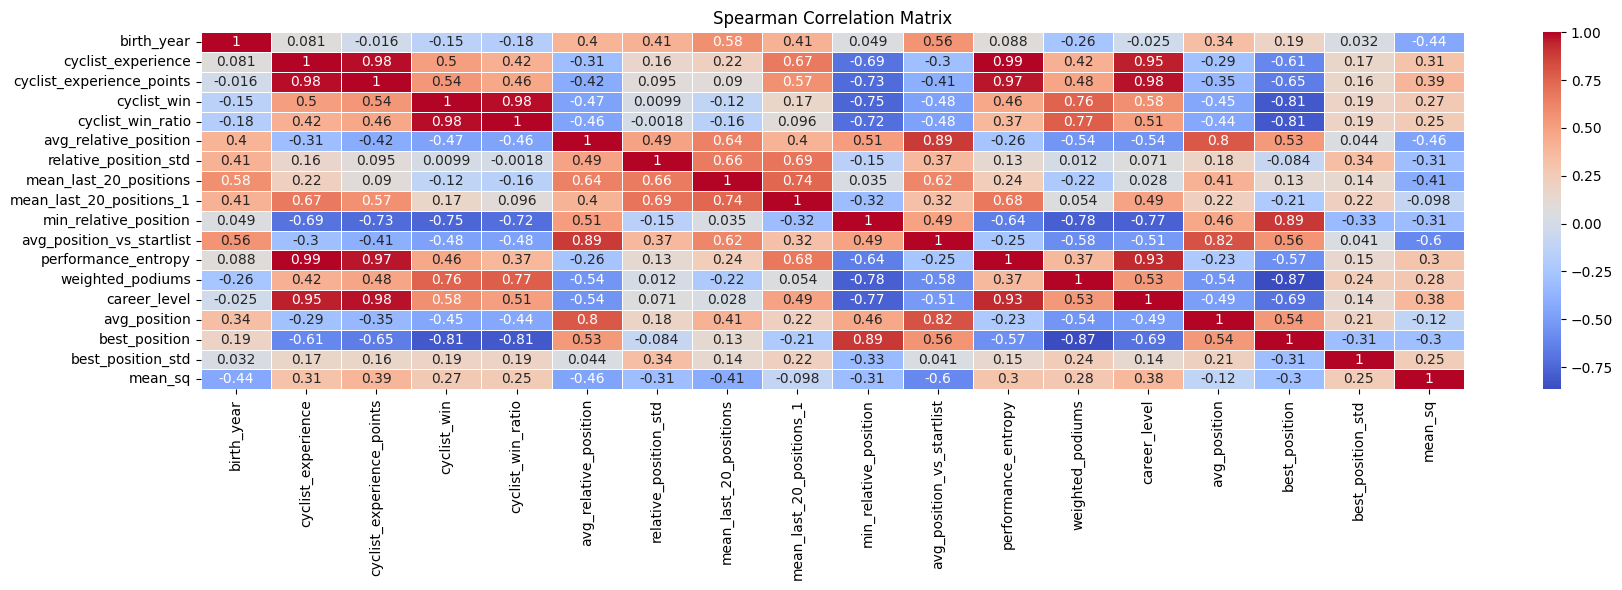
\includegraphics[width=1\textwidth]{images/DE/correlation.png}
\caption{\small Spearman Correlation Analysis on Cyclist Dataset}
\label{fig:cyclists_feature_correlation}
\end{figure}

\subsection{Correlation}

\autoref{fig:cyclists_feature_correlation} presents a correlation plot of the engineered features. While Kendall-based correlations are also available in the notebook, we chose to focus on Spearman correlations. Spearman correlations often exhibit similar trends but yield higher values, treating features as more correlated. This makes them more suitable for the next clustering step, where it is important to select features with limited correlation.



\section{Clustering}
An iterative process was employed to evaluate various feature configurations for clustering. Each configuration involved outlier detection, clustering, and subsequent analysis to interpret and characterize the resulting clusters. This approach enabled the identification of the most meaningful features to optimize clustering performance.
After several iterations, the three key features selected were: \textit{avg\_relative\_position}, \textit{mean\_sq}, and \textit{career\_level}. Using these features, our goal was to achieve a clustering that would allow us to identify groups of cyclists based on their cycling performance, considering how well a cyclist has positioned himself, how much he has competed in his career, and how important the races he has competed in have been. 
To obtain comparable results, we used the same three features with all clustering algorithms finding out that K-Means delivered the best results according to our characterization goal.
In the following sections, we provide an overview of the entire process.

\subsection{Outlier Detection}
Outlier detection was essential to ensure that extreme values or outliers did not significantly affect the clustering results, allowing more accurate and meaningful groupings. Three different techniques were employed:
\begin{itemize}
    \vspace{-0.20cm}
    \item \textbf{One-class SVM}: it identified 120 outliers
    \vspace{-0.20cm}
    \item \textbf{Connectivity Approach}: it identified 107 outliers 
    \vspace{-0.20cm}
    \item \textbf{Isolation Forest}: it identified 89 outliers
\end{itemize}
\vspace{-0.20cm}

\noindent
Finally, we implemented a customized strategy by combining the results of these methods in an ensemble fashion. Specifically, we adopted a majority voting approach: rows identified as outliers by at least two methods were excluded from the dataset. Through this approach, 70 outliers were identified, and removed; results are shown in \autoref{fig:outlier}.

\begin{figure}[H]
\centering
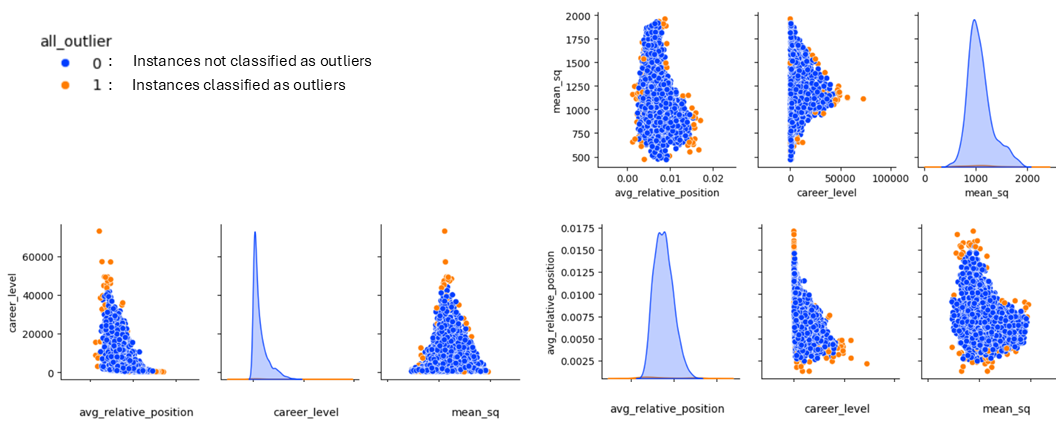
\includegraphics[width=0.9\textwidth]{images/CLUSTER/outlier.png}
\caption{ \small Outliers identified using majority voting ensemble approach\small }
\label{fig:outlier}
\end{figure}


%---------------------------------------------------------
\subsection{K-means Clustering}
\subsubsection{Preprocessing, Best K, and Visualization}

Initially, all the selected features were scaled to have zero mean and unitary standard deviation. This preprocessing step is essential as it improves the performance of the K-means algorithm, which is sensitive to the scale of the input features. \\

\noindent
\textbf{Best K Parameter Search}\\
A grid search was conducted to test different configurations of the parameter k (number of clusters). For each configuration, we plotted the SSE, Silhouette, and Davies-Bouldin scores to monitor clustering performance. While these plots provided valuable insights, the final choice of k was not only based on them.
Since clustering is an exploratory process and good metric scores do not always guarantee that clusters align with our expectations or domain-specific needs, we also performed cluster characterization for various k values to evaluate different results more empirically.
Therefore, the decision for the optimal k was made by combining the analysis of the metrics in \autoref{fig:metrics_kmeans} with the evaluation of the characterization and significance of the clusters finding \textbf{k=3} as best k.\\

\begin{figure}[H]
    \centering
    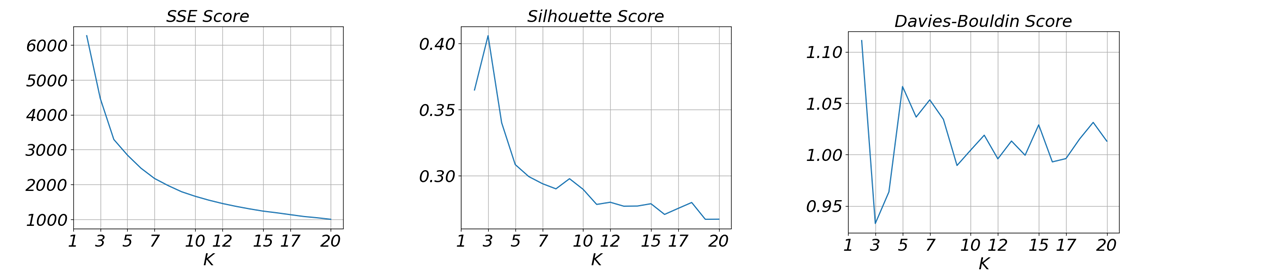
\includegraphics[width=1\textwidth]{images/CLUSTER/k-means/metrics.png}
    \caption{ \small Trends of K-means SSE, Silhouette, and Davies-Bouldin scores as the number of clusters \( k \) increases.}
    \label{fig:metrics_kmeans}
\end{figure}

\noindent
\textbf{Visualization Analysis}\\
From the pair plot and PCA plot in \autoref{fig:pairplot_kmeans}, one can observe that clusters are generally well separated. However, some overlaps are visible indicating that while the clustering captures the overall structure of the data effectively, some degree of variability or noise remains. These overlaps suggest that the boundaries between clusters are not entirely rigid, likely reflecting the inherent complexity or overlapping characteristics of the dataset.

\begin{figure}[H]
\centering
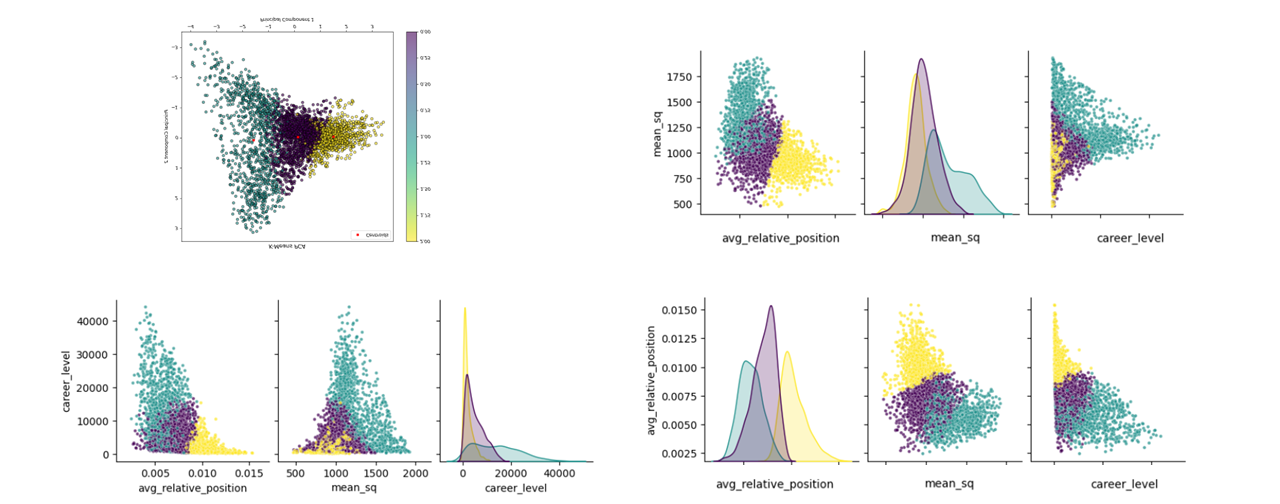
\includegraphics[width=0.9\textwidth]{images/CLUSTER/k-means/pairplot.png}
\caption{ \small K-means feature pair plots and PCA visualization \small }
\label{fig:pairplot_kmeans}
\end{figure}

\subsubsection{Characterization}
Starting by examining the Parallel Coordinates Plot for Centroids in \autoref{fig:cluster_centroids}, we have an overview of the identified clusters that are characterized as follows:

\vspace{-0.2cm}

\begin{itemize}
    \item \textbf{Cluster 0}: \textit{Intermediate Cyclists}
    \vspace{-0.2cm}
    \item \textbf{Cluster 1}: \textit{Best Cyclists}
    \vspace{-0.2cm}
    \item \textbf{Cluster 2}: \textit{Worst Cyclists}
\end{itemize}

\vspace{-0.2cm}


\begin{figure}[H]
\centering
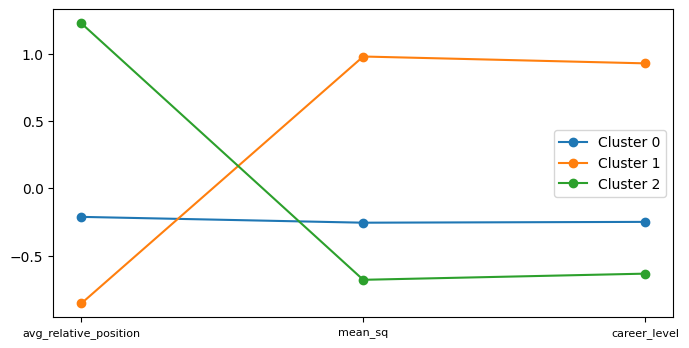
\includegraphics[width=0.5\textwidth]{images/CLUSTER/k-means/Centroids_plot.png}
\caption{ \small \small K-means Parallel Coordinates Plot for Centroids}
\label{fig:cluster_centroids}
\end{figure}

\noindent
The cyclists in the \textit{Best Cyclists} cluster have a low average relative position (meaning they often finish among the top), high average start list quality, and a high career level. In contrast, cyclists in the \textit{Worst Cyclists} cluster show the opposite values. Those in the \textit{Intermediate Cyclists} cluster fall somewhere in between.
Further analysis of the mean values of each feature across clusters aligns with the patterns observed in the \autoref{fig:cluster_centroids}, confirming consistent trends for features such as career level, mean start list quality, and average relative position.\\

\noindent
\textbf{Insights from Non-Clustering Features}

\noindent
We then analyzed the distributions of additional features that were not directly used with the clustering algorithms but provided valuable insights into cyclist's quality and experience. Examining these distributions ensures that the clusters are accurately interpreted and align with the expected performance levels that emerged during the characterization process.

%---- WEIGHTED PODIUMS
The distribution of \textbf{weighted podiums} reveals distinct patterns across the clusters. In the first plot of \autoref{fig:podiums_distr_kmenas}, a significant proportion of cyclists have a weighted podium count of 0, with a sharp decline as the count increases slightly. Conversely, in the second and third plots, corresponding to higher-ranked cyclists, the decline is more gradual. This trend illustrates the superior ability of cyclists in these clusters to consistently achieve higher placements.  

\begin{figure}[H]  
\centering  
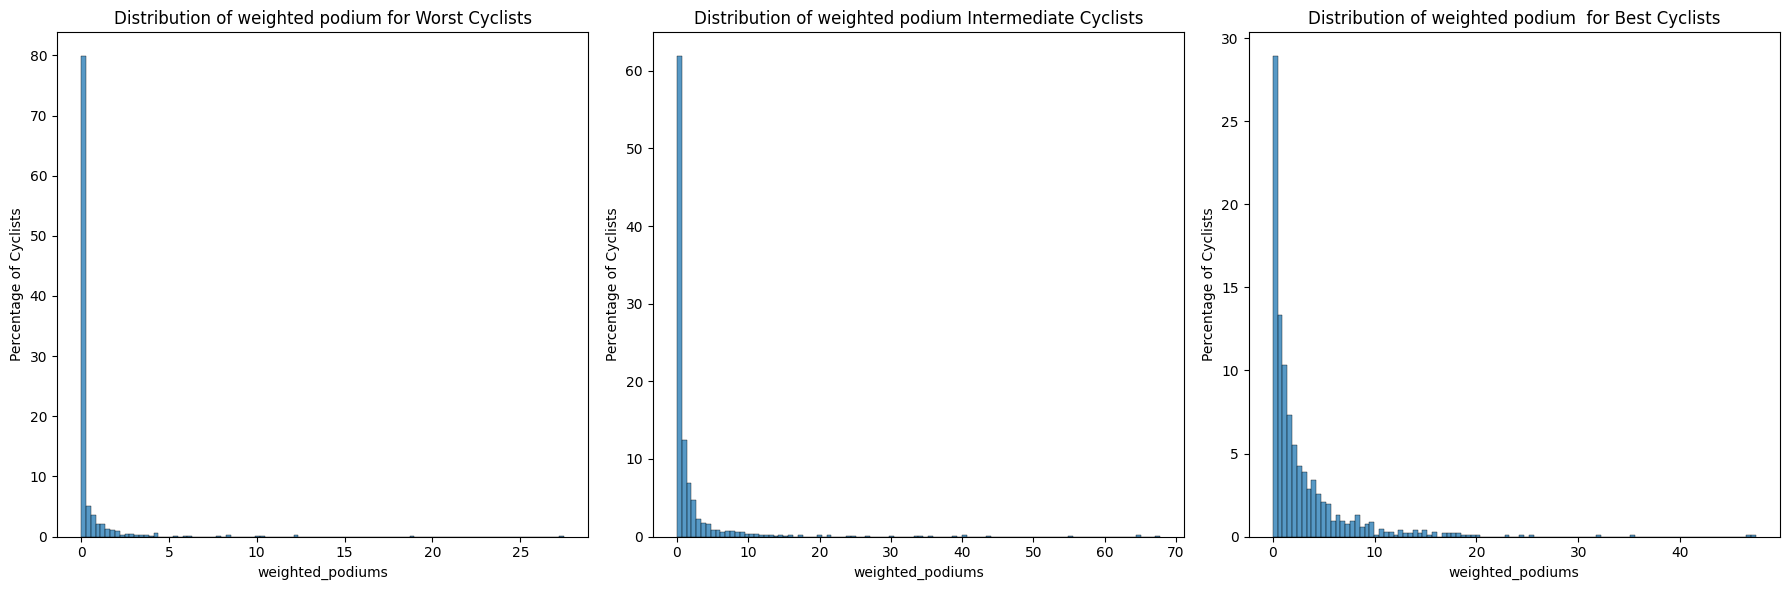
\includegraphics[width=0.93\textwidth]{images/CLUSTER/k-means/podiums_distr.png}  
\caption{ \small K-means weighted podiums distribution, with cyclists represented as percentage}  
\label{fig:podiums_distr_kmenas}  
\end{figure}  

\noindent  
\textbf{Cyclist experience} also demonstrates an expected progression across clusters. As shown in \autoref{fig:experience_distr_kmenas}, the percentage of highly experienced cyclists rises as we move from the worst-performing cluster to the best-performing one. This pattern aligns with expectations, reinforcing the notion that experience correlates with superior performance.  

\begin{figure}[H]  
\centering  
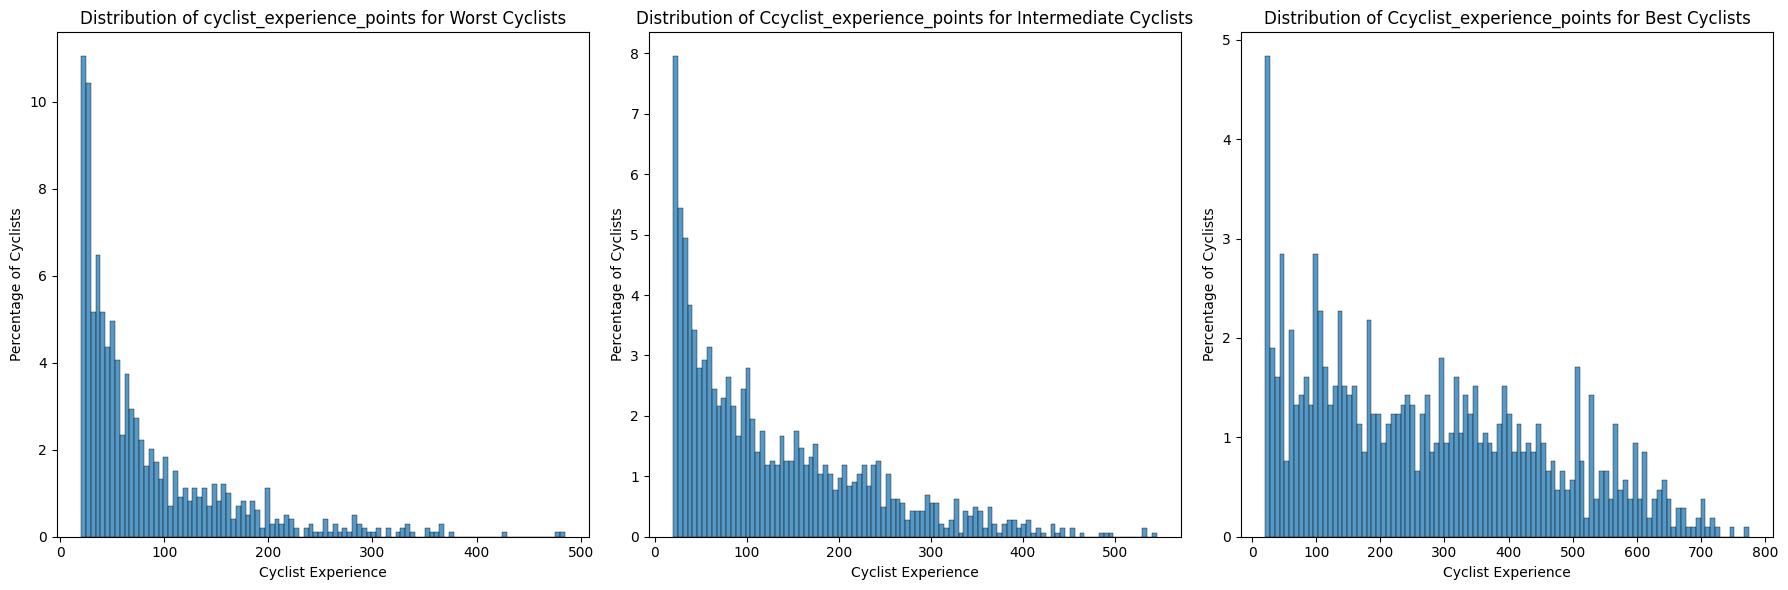
\includegraphics[width=0.93\textwidth]{images/CLUSTER/k-means/experience_distr.png}  
\caption{ \small K-means cyclist experience distribution, with cyclists represented as percentage}  
\label{fig:experience_distr_kmenas}  
\end{figure}  

\noindent  
Examining the \textbf{best position} achieved by cyclists, a clear distinction emerges across clusters. Figure \ref{fig:best_position_distr_kmeans} highlights that as we transition from the worst-performing cluster to the best, the proportion of cyclists achieving top positions increases significantly, while the percentage of those with lower rankings as best positioning decreases.  

\begin{figure}[H]  
\centering  
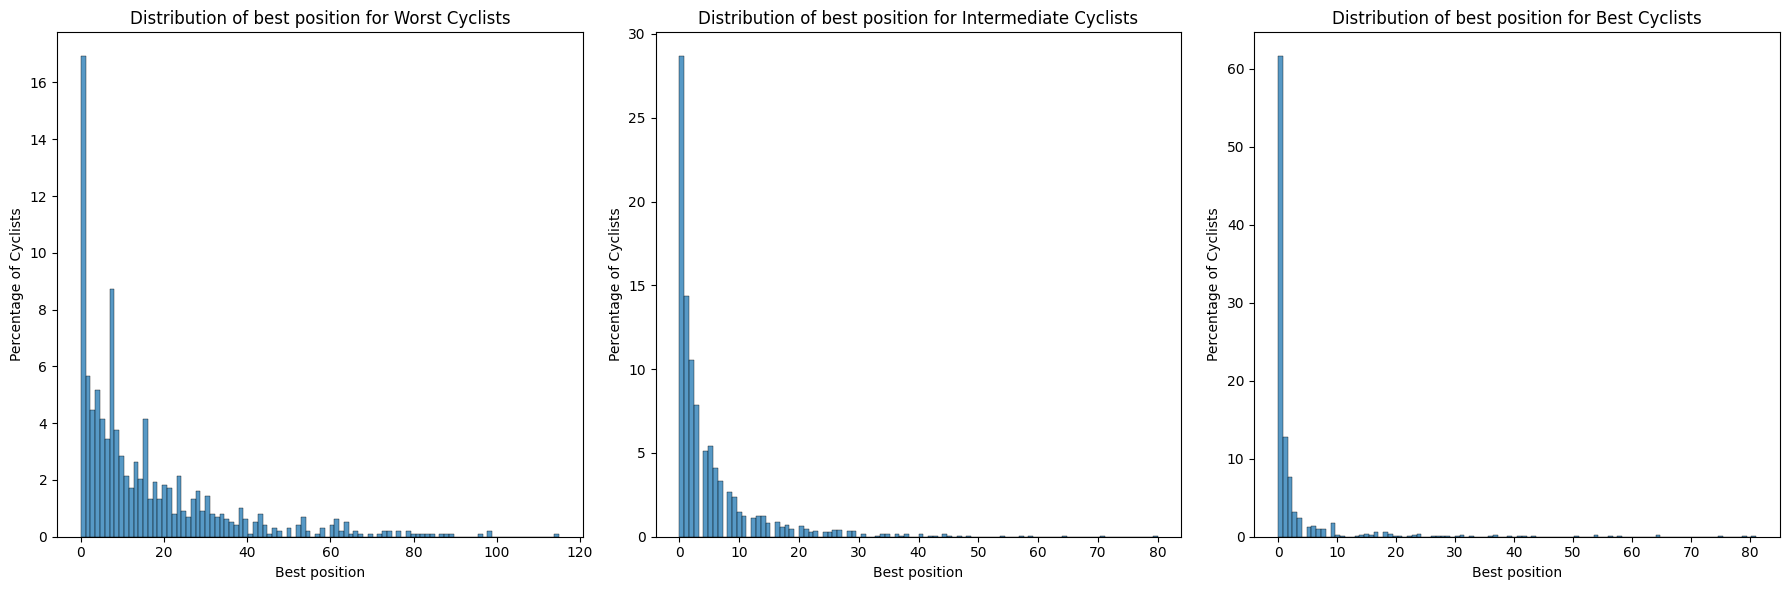
\includegraphics[width=0.93\textwidth]{images/CLUSTER/k-means/best_position_distr.png}  
\caption{ \small K-means best position distribution, with cyclists represented as percentage}  
\label{fig:best_position_distr_kmeans}  
\end{figure}  

\noindent  
\textbf{Performance entropy} shows a slight increase among higher-performing clusters, as illustrated in \autoref{fig:performance_entropy_distr_kmeans}. This result, while counterintuitive at first glance, can be explained by the larger number of races participated in by top cyclists, including high-level ones. Such extensive participation introduces variability in their results. In contrast, lower-level cyclists often compete in fewer races, leading to more consistent but less remarkable performances.  

\begin{figure}[H]  
\centering  
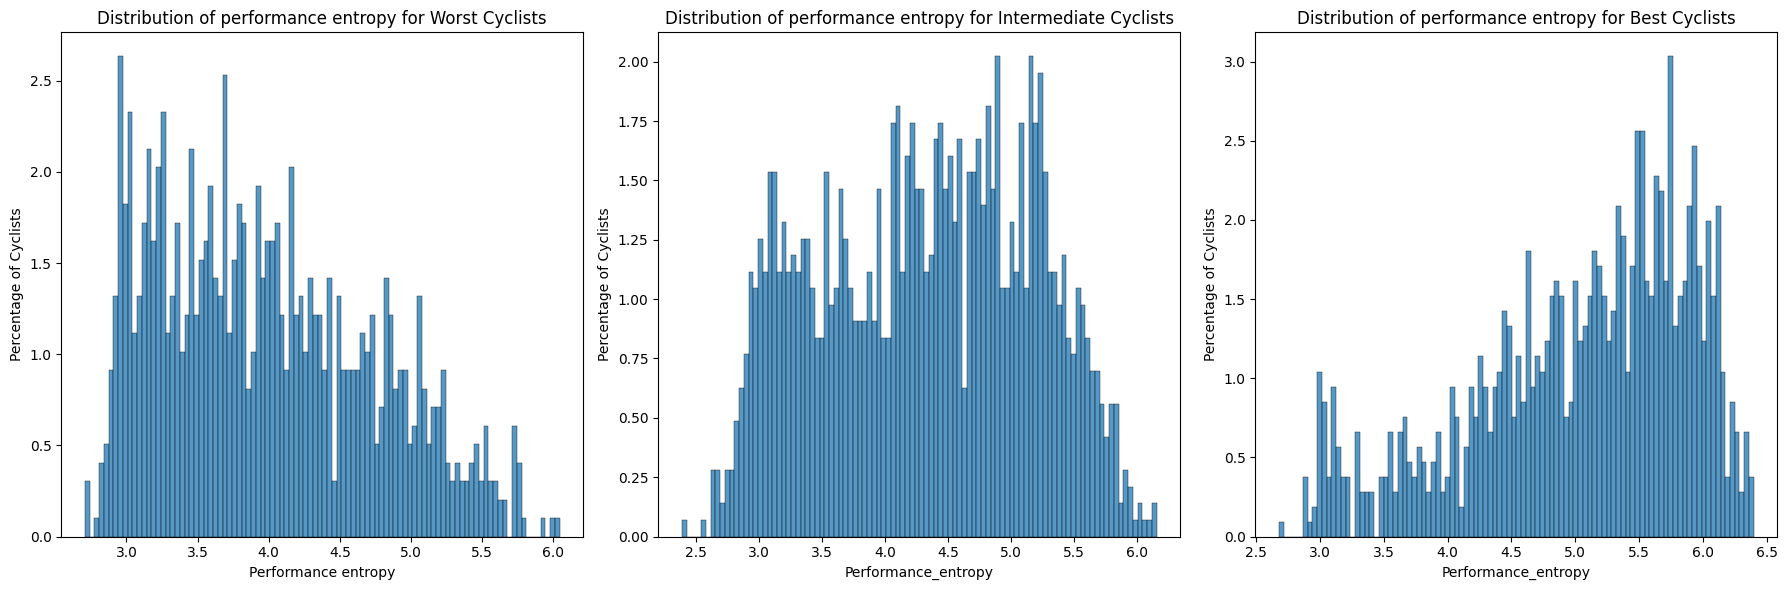
\includegraphics[width=0.93\textwidth]{images/CLUSTER/k-means/performance_entropy_distr.png}  
\caption{ \small K-means performance entropy distribution, with cyclists represented as percentage}  
\label{fig:performance_entropy_distr_kmeans}  
\end{figure}  


\noindent
\textbf{Final Analysis and Conclusions}\\
The identified clusters exhibit feature distributions that align with our expectations of a cyclist’s skill level confirming that K-means effectively groups cyclists based on their skill levels. Despite this, the distributions of extra-clustering features reveal that the classes are not perfectly separated into distinct bins. High or low values of certain features can still be observed in clusters where they would not be expected.

We can also notice that skill level is determined not only by strong race results, weighted by the importance of the competitions, but also by career activity. Incorporating the career level feature allowed the clustering to identify a "rank" that accounts for both performance and participation throughout a cyclist’s career.  

As a result, a cyclist who has competed in only a few races and won them all may not be classified among the best. This is because the career level feature factors in the total number of completed races and the cumulative score, weighted by race importance. \\

\noindent
\textbf{Summary:}    

\begin{itemize}
    \vspace{-0.20cm}
    \item \textbf{Best Cyclists cluster}: Cyclists who achieved excellent average results, with many podiums and extensive experience in high-level races.
    \vspace{-0.20cm}
    \item \textbf{Intermediate Cyclists cluster}: Cyclists with a good number of races and discrete average results, with experience in medium-level races.
    \vspace{-0.20cm}
    \item \textbf{Worst Cyclists cluster}: Cyclists who achieved generally poor results in low-level races and/or have limited experience.
\end{itemize}

We want also to highlight that another configuration of features was tested with K-means using \textit{mean\_last\_20\_position} instead of \textit{mean\_sq}. This was because we wanted to include information related to underperformance as well. The results obtained are significant, but not as optimal as those of the first feature configuration. All the details are in the notebook \texttt{TASK\_3/k\_means.ipynb}.

%---------------------------------------------------------


\subsection{X-means}
X-means provides a fairly clear separation between the clusters of worst, intermediate, and best cyclists with a slightly lower level of accuracy than K-means. In \autoref{fig:pairplot_xmeans} we can see PCA and pair plot.

\begin{figure}[H]
\centering
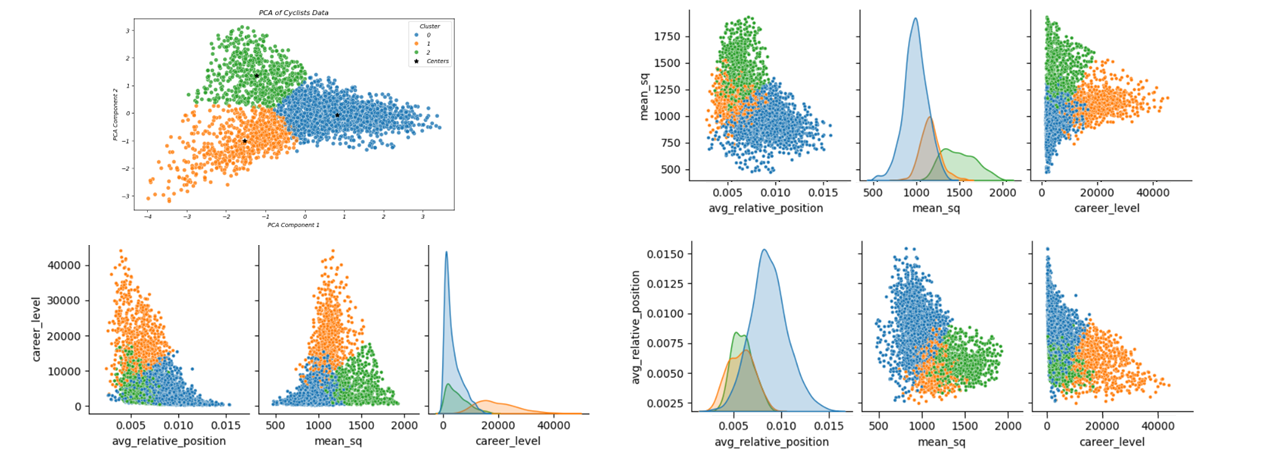
\includegraphics[width=0.93\textwidth]{images/CLUSTER/X-means/pairplot.png}
\caption{ \small  X-means feature pair plots and PCA visualization \small}
\label{fig:pairplot_xmeans}
\end{figure}

\subsubsection{Characterization}

After full characterization (the same as used for K-means), the clusters were mapped as follows: \textbf{cluster 0 = worst cyclists}, \textbf{cluster 1 = best cyclists}, and \textbf{cluster 2 = intermediate cyclists}. We can observe some key features through an initial analysis of the plot of the centroid values shown in the \autoref{fig:cluster_centroids_xmeans}.
For the intermediate cyclists cluster, the centroid value of \textit{start\_list\_quality} is significantly higher than that of the worst cyclists cluster. We can also notice that the difference in average position between intermediate and top cyclists clusters is almost negligible. In the end, the \textit{career\_level} of the intermediate cyclists cluster is very close to that of the worst cyclists cluster.\\

\noindent
The rest of the characterization yielded results similar to those of K-means, although not identical. From this, we made the following observations:
\begin{enumerate}
    \item \textbf{Worst Cyclists Cluster}: cyclists who have participated in relatively fewer races on average compared to the best cyclist cluster, achieving high (so not good) placements in low-importance races.

    \item \textbf{Best Cyclists Cluster}:  
    in this cluster, some cyclists have competed in a large number of races (which is the reason why they have a very high \textit{career\_level} value) and have achieved good placements on average slightly better than those of the cyclists in the intermediate cluster. The average start list quality is quite low compared to the intermediate cluster, which means that despite competing in many races, many of them were not always at a high level.

    \item \textbf{Cluster Intermediate Cyclists}:  
    in this cluster, some cyclists have participated in a relatively small number of races compared to the best cyclists cluster (unlike K-means, X-means shows a larger experience gap between these two clusters) but they have achieved good placements and have competed in high-level races.
\end{enumerate}

\noindent
\textbf{Summary}
\begin{itemize}
    \item \textbf{Worst Cyclists Cluster}: represents the worst cyclists in terms of experience, results, and career level.
    \item \textbf{Intermediate Cyclists Cluster}: includes cyclists with not-so-high experience but great results in high-quality races.
    \item \textbf{Best Cyclists Cluster}: includes cyclists with the best average results compared to other clusters (slightly better than the intermediates), high experience, and a high career level but a low \textit{mean\_sq} value.
\end{itemize}

\begin{figure}[H]
\centering
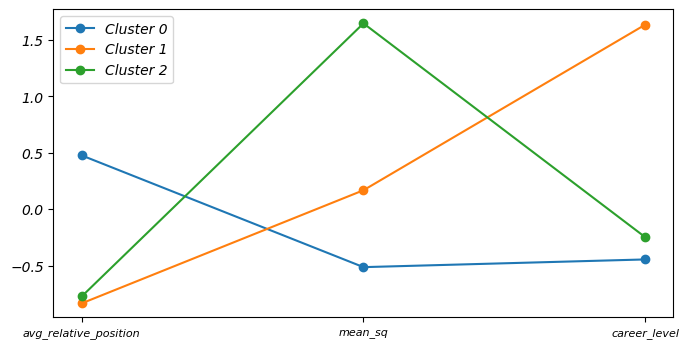
\includegraphics[width=0.5\textwidth]{images/CLUSTER/X-means/centroids_plot.png}
\caption{ \small \small Parallel Coordinates Plot for X-means Centroids}
\label{fig:cluster_centroids_xmeans}
\end{figure}

\noindent
In general, we can say that the results obtained are fairly interpretable but slightly more confusing compared to those from K-means.

%--------------------------------------------------- 
\subsection{Hierarchical Clustering}
We performed an agglomerative hierarchical clustering on the same features highlighted in the previous sections. \\

\subsubsection{Best Parameters Search}
To find a suitable configuration, we searched all possible combinations of metrics and associated methods, testing several cluster numbers of 3, 4, 5, 6, and 10 for each. Finally we calculated the silhouette and DB scores to assess them. We sorted the results by decreasing silhouette and increasing DB scores and looked at the top twenty configurations. We then explored each one by hand and found that the one that came closest to our needs used \texttt{correlation} as metric with \texttt{average} method and found 3 clusters with a 0.35 as silhouette score and 1.09 as DB score. \\

\subsubsection{Characterization}
As one can see from \autoref{fig:hier-plots} the algorithm identified three distinct clusters. The dendrogram on the left shows the hierarchical clustering of the data based on correlation distance and the average linkage method. The leftmost cluster is more separated from the other two, indicating a higher dissimilarity. The remaining two clusters are more closely grouped, suggesting that they may share similar characteristics.

\begin{figure}[H]
    \centering
    \begin{subfigure}[b]{0.33\textwidth}
        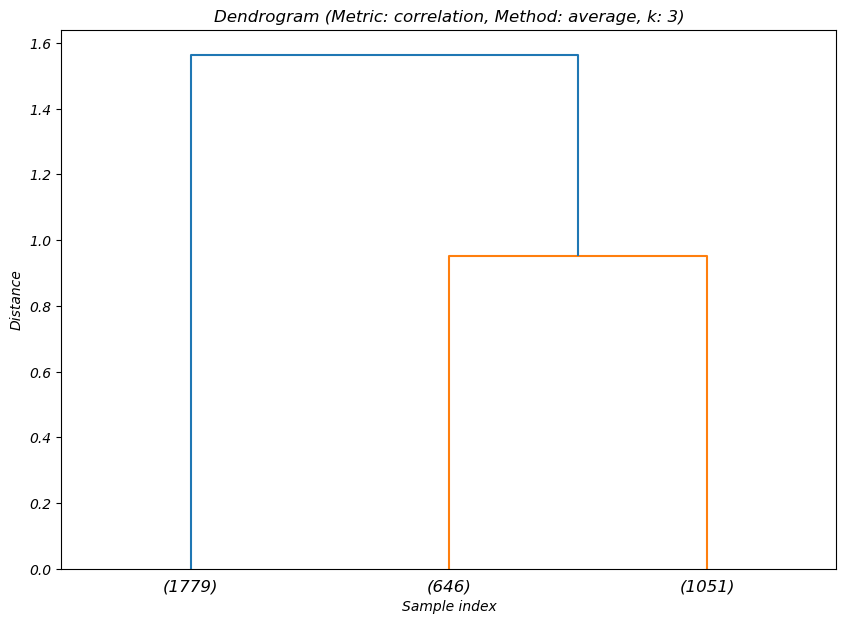
\includegraphics[width=\textwidth]{images/CLUSTER/hierarchical/dendogram.png}
    \end{subfigure}
    \begin{subfigure}[b]{0.33\textwidth}
        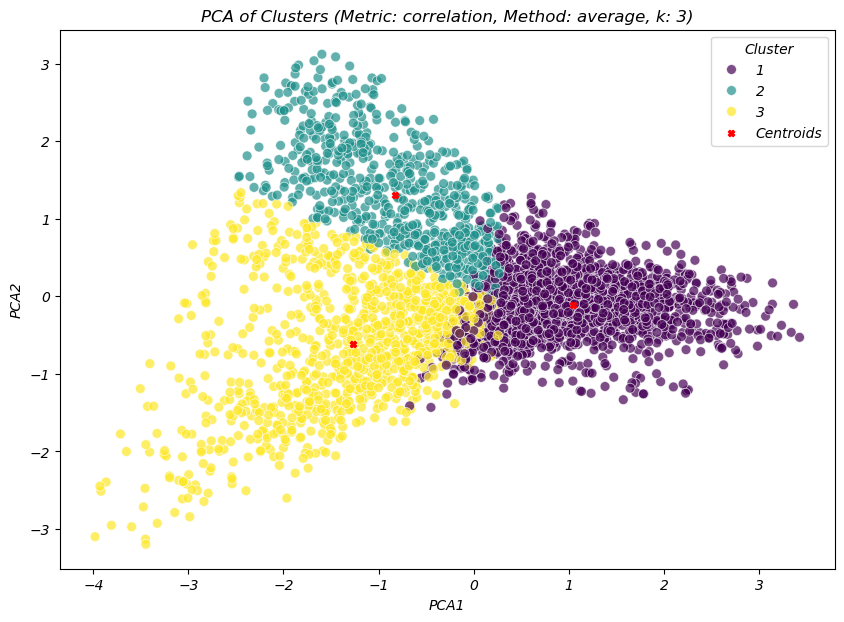
\includegraphics[width=\textwidth]{images/CLUSTER/hierarchical/pca.png}

    \end{subfigure}
    \begin{subfigure}[b]{0.5\textwidth}
        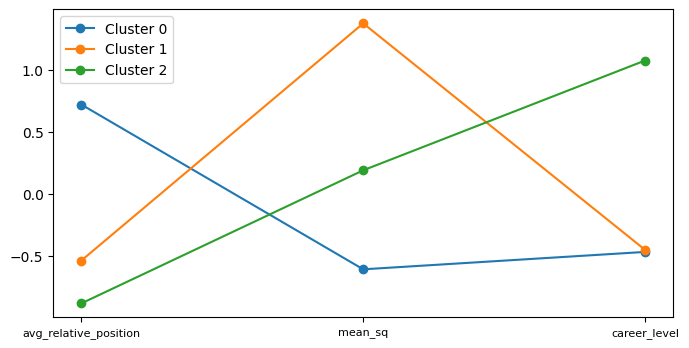
\includegraphics[width=\textwidth]{images/CLUSTER/hierarchical/coordinates_hier.png}
    \end{subfigure}
    \caption{ \small From left to right: Dendogram, 2D PCA and Parallel Coordinates Plot for hierarchical clusters computed centroids }
    \label{fig:hier-plots}
\end{figure}

\noindent From the Parallel Coordinates Plot, we hypothesized that: \textbf{Cluster 0} might group the worst cyclists (very low average relative position, a medium mean start list quality, and a very high career level, \textbf{Cluster 1} the intermediate ones (slightly higher career level than those in \textbf{Cluster 0}, but with a lower average relative position and the highest start list quality in the clustering) and finally the \textbf{Cluster 2} the best ones (very low average relative position, a medium mean start list quality, and a very high career level). Overall, results are very similar to the one obtained with X-means.

To check if our hypothesis held, we plotted the distributions of \textit{weighted\_podiums}, \\\textit{cyclist\_experience} and \textit{performance\_entropy} in each cluster found. The worst cyclists typically show low or null podiums, the best cyclists show higher feature values and intermediate cyclists fall in between, with some overlap. Although this overlap is minimal, we find the interpretation less clear than in K-Means where the subdivision was clearer. The distribution of experience is similar in the worst and intermediate clusters, but the best cyclists have much higher average experience, correlating with a higher career level. The percentage of cyclists with higher performance entropy increases slightly from the worst to the best cyclists. This is due to higher-performing cyclists participating in more races, leading to more fluctuating results. In contrast, lower-performing cyclists tend to have fewer races, resulting in more regular performance with fewer peaks. \\

\noindent\textbf{Conclusion}\\
Although the final result is the similar to K-means, we believe that K-means is better at grouping riders based on their overall performance.

\subsection{DB-Scan Clustering}
The DB-Scan clustering was the poorest one in terms of result quality. The following sections describe the process.\\

\noindent\textbf{Best Parameters Search}\\
To optimize the clustering process, we started constructing the distance matrix for the scaled dataset and identifying the 5 nearest neighbors for each data point. Leveraging the Kneedle library for the elbow method, we found the critical elbow in the sorted distance curve. We then tested different values for \texttt{min\_samples} (5, 7, 10, 12, 15, 20, 25, 30, 50, 80) and \texttt{epsilon}, selecting 200 linearly spaced values between 0.01 and 1. The best DBSCAN fit found only one cluster with all the data, which wasn't surprising given the data's lack of dense, disconnected structures. In a second trial, after analyzing results with more than one cluster, the best result came from \texttt{min\_samples} = 12 and \texttt{eps} = 0.065, yielding 2 clusters and outliers. However, as observed in \autoref{fig:dbscan-pca}, the results were not promising.

\begin{figure}[h]
    \centering
    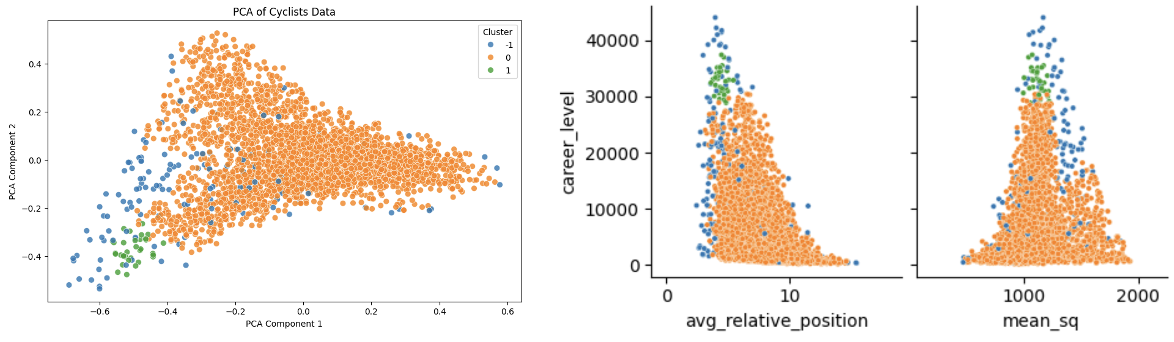
\includegraphics[width=0.8\linewidth]{images/CLUSTER/dbscan/pca.png}
    \caption{ \small DBSCAN Pairlplot and PCA}
    \label{fig:dbscan-pca}
\end{figure}

\noindent We found that cyclists in \textbf{Cluster 1} (the best cluster) had won at least one stage, while most in \textbf{Cluster 0} had not. Surprisingly, 75\% of the cyclists in the outlier cluster won at least one stage, suggesting outliers may be high-performance cyclists. This cluster also includes cyclists with both high and low experience levels. Top cyclists show higher performance variability, likely due to their greater experience and participation in more stages. When considering career levels, \textbf{Cluster 1} represents the best cyclists, though some are in \textbf{Cluster 0}'s tail and many in the outliers cluster, which also contains cyclists with low experience and career levels due to the distribution of professionals.\\

\noindent\textbf{Conclusion}\\
Overall, \textbf{Cluster 1} contains cyclists with higher career levels, more experience, and more wins, along with better race positions and greater variability. These cyclists' superior performance is linked to extensive racing experience. The \textbf{Cluster 0} tries to group the rest. We think that the clustering quality does not match K-Means.

\subsection{Comparison of metrics}
From Table \ref{tab:clustering_results}, we can observe that K-means and X-means achieve the best results, with the lowest Davies-Bouldin scores and highest Silhouette scores, indicating well-separated and compact clusters. These findings align with their strong performance during cluster characterization.

While X-means slightly outperforms K-means in compactness and separation, K-means offers greater clarity and precision in cluster characterization.

\begin{table}[H]
    \centering
    \scriptsize
    \begin{tabular}{p{2.0cm}ccccccc}
    \toprule
    \textbf{Model} & \textbf{SSE} & \textbf{Silhouette} & \textbf{Davies-Bouldin Score} \\
    \midrule
    \textbf{K-means} 
      & 4468
      & 0.40
      & 0.93 \\
    \textbf{X-means} 
      & 4535
      & 0.41
      & 0.86 \\
    \textbf{DBSCAN} 
      & -
      & 0.29
      & 1.54\\
    \textbf{Hierarchical} 
      & -
      & 0.35
      & 1.09 \\
    \bottomrule
    \end{tabular}
    \caption{ \small \small Cluster Algorithm Metrics Comparison}
    \label{tab:clustering_results}
\end{table} 

\section{Prediction}
The goal of the task is to fit a prediction model that will predict the final position of a given cyclist in a race, discriminating those cyclists whose placement is in the top 20 (class 1) positions from the others (class 0). To pursue this goal, we revamped the data cleaning and feature engineering tasks to prepare the races dataset for classification.

\subsection{Data Cleaning}
First, we eliminated those stages associated with a null \textit{climb\_total} or \textit{profile} feature value. Since we used those features to engineer new ones, we avoided dealing with null values. This operation dropped $180'556$ of $589'616$ total rows. On a professor's advice, we also eliminated the stages with less than 25 participants to avoid non-representative data, as smaller group sizes could disproportionately affect the distinction between the top 20 cyclists and non-top 20 cyclists. To facilitate this operation, we counted how many cyclists each stage had adding this information to the dataset.

\subsection{Feature Engineering}
We engineered some new features the task can rely on. Below you can find a detailed overview. \\

\noindent
\textbf{top\_20}: this feature represents the classification label: 1 if the position associated with a cyclist is smaller or equal to 20 and 0 otherwise.\\ \\
Some basic statistics run on this column made us aware of an important dataset-related thing: the unbalance. Class 0 represents 87\% of the entire dataset while class 1 only has 13\%. In the next section, we will consider some of the issues related to this problem. \\

\noindent
\textbf{cyclist\_level}: this feature quantifies the level of a cyclist considering all the placements until the stage for which we are calculating the feature. This feature is calculated using the method described in \autoref{sec:feat_eng}. \\

\noindent
\textbf{cyclist\_experience}: this feature counts the number of stages a cyclist participated in until the stage for which we calculate the feature. \\

\noindent
\textbf{avg\_relative\_position}: this feature represents the average positioning of the cyclist and it's calculated as described in \autoref{sec:feat_eng}, with the distinction that it is computed up to, but excluding the current stage. \\

\noindent
\textbf{avg\_relative\_position\_profile}: this feature expresses the average relative position reached by a cyclist in a specific race's profile until the stage for which we calculate the feature. \\

\noindent
\textbf{rel\_position\_length}: this feature expresses the relative position reached by a cyclist in a particular class of race's length i.e. 0 (short), 1 (medium), 2 (long) until the stage for which we are calculating the feature. \\

\noindent
\textbf{rel\_position\_climb}: this feature represents the average relative position reached by a cyclist in a race taking into account a particular race climb until the stage for which we are calculating the feature. To do this we defined three classes of climbs: 0 (flat/low climb), 1 (hilly/medium climb), and 2 (mountainous/high climb). \\

\noindent
\textbf{avg\_cyclist\_level}: this feature replaces the \textit{startlist\_quality} feature. It expresses the same idea but is calculated using our engineered feature \textit{cyclist\_level}.\\

\noindent
\textbf{position\_entropy}: this feature expresses the entropy of a cyclist's position in all the stages until the one for which the feature is computed.\\

\noindent
\textbf{top\_20\_entropy}: same reasoning as the previous feature but related to the top 20: the higher the entropy the more unpredictable the positioning in the first position is. \\

\noindent At the end of the process, there were 32 total columns in the dataset.

\subsubsection{Feature Correlation}
We analyzed correlations before splitting the dataset into training, validation, and test sets.

\noindent As one can see from the Figure \ref{fig:class-correlations} there are some high-correlated features, which are: \textit{climb\_total}, \textit{profile}, \textit{cyclist\_age}, \textit{cyclist\_level}, \textit{cyclist\_experience}, \textit{relative\_position}, \textit{avg\_relative\_position}, \\ \textit{cyclist\_experience\_profile}, \textit{cyclist\_experience\_length}, \textit{avg\_rel\_position\_climb}, \textit{position\_entropy}.

Most correlations were expected since they occur between features used to engineer others. Of course, since we cannot deal with highly correlated features during the classification, we decided to select only a subset of non-correlated features.


\subsection{The imbalance dataset problem}
\label{subsec:imbalancing}
Building a binary classifier on an imbalanced dataset like ours poses significant challenges. The dataset reflects a real scenario, with only a small percentage of cyclists in the top 20, leading to potential classifier bias toward the majority class, which comprises 84\% of the data. Simple models risk predicting not-top 20 for all inputs, failing to capture minority class patterns and generalize effectively, which may lead to overfitting. Misleading metrics like accuracy emphasize the dominance of the majority class, making alternatives like the f1-score more suitable. Considering the significant class imbalance in the dataset and the critical importance of class 1 to class 0, we chose to optimize the models based on the standard F1-score.

\begin{figure}[H]
    \centering
    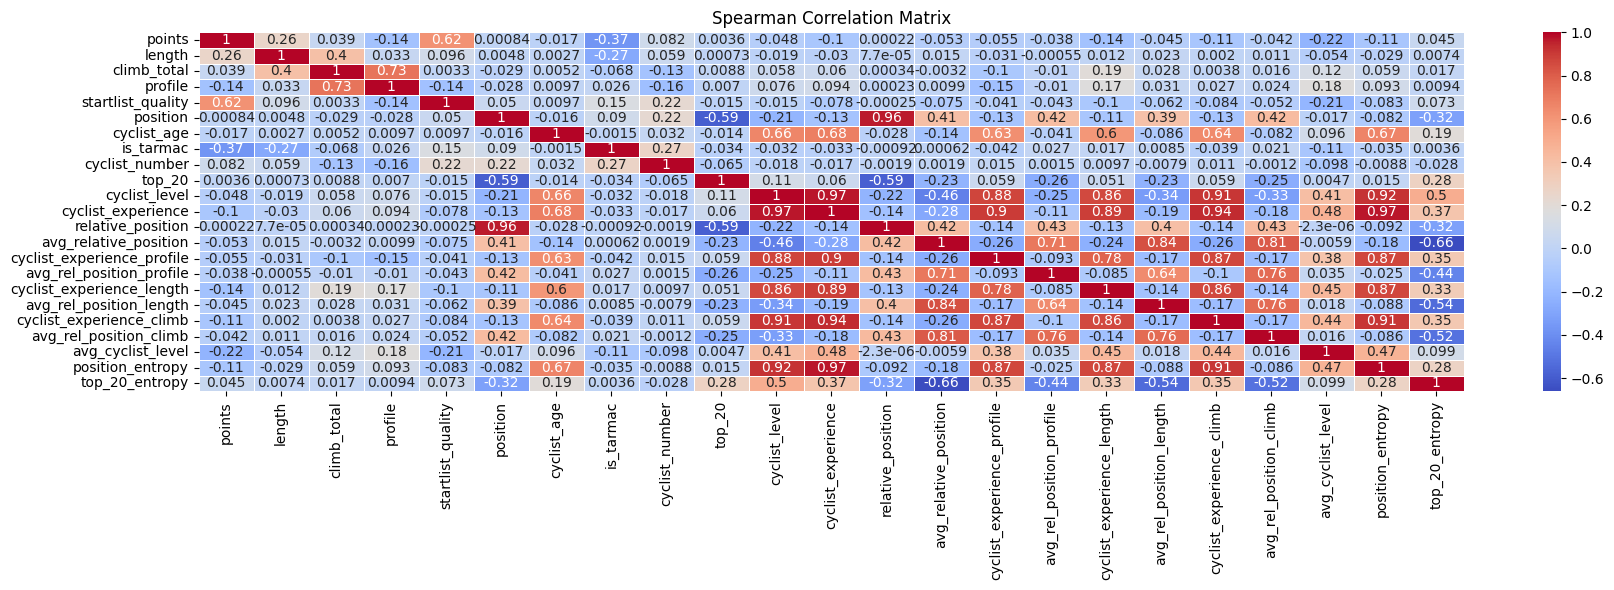
\includegraphics[width=0.88\linewidth]{images/CLASSIFICATION/correlations.png}
    \caption{\small Correlation between numerical features during feature engineering process for the classification}
    \label{fig:class-correlations}
\end{figure}




\subsection{Task Complexity and Classification Challenges}
\label{subsec:extra_analysis}
The extra analysis (\enquote{\texttt{TASK\_5/extra\_analyis.ipynb}}) highlights the inherent challenges of the classification task, emphasizing that the dataset and the nature of the problem make achieving reliable predictions difficult. First, the extra analysis reveals overlapping class distributions in 2D and 3D feature spaces, further complicating classification. Mutual information values for features are low, indicating weak predictive power. To further investigate, we shuffled the labels to simulate a random dataset and compared the results with our model's performance. The model’s slightly better performance suggests weak but present patterns that are difficult to capture effectively.
Further complicating the task is the strategic nature of cycling, which impacts the dataset's structure and predictive potential. In races like the Giro d’Italia, overall success is determined by accumulated time rather than consistent stage victories. Cyclists aiming for the general classification often adopt strategies such as prioritizing minimal time losses in crucial stages while finishing in lower positions in others, sometimes as far back as 100th place, to conserve energy or focus on more critical stages in tightly scheduled races. These strategic decisions, influenced by factors such as team support, energy conservation, and tactical positioning, introduce variability that makes stage-level results context-dependent. Additionally, variables like weather, terrain, and race dynamics are absent from the dataset and add unpredictability, further complicating the task.
To validate this, we analyzed cyclists who achieved victories or top finishes in prestigious races like the Giro d’Italia and the Tour de France. Despite their overall success, these cyclists often recorded significantly low positions in individual stages, underscoring the challenge of relying solely on stage-level results. While not a rigorous statistical demonstration, this analysis supports the conclusion that the task, as formulated, struggles to encapsulate the complexities of cycling, making accurate classification inherently difficult.

\subsection{Our approach to the task}
We employed a multi-model training approach, with the analysis focused on: Naive-Bayes, Logistic Regression, K-NN, Decision Tree, SVM, Random Forest, Gradient Boosting Machine, Neural Network, and Rule-Based Classifier. We optimized each model using hyperparameter searches, various feature combinations, and sampling strategies. After testing various feature subsets, we selected \textit{climb\_total}, \textit{cyclist\_age}, \textit{cyclist\_level}, \textit{cyclist\_experience}, \textit{avg\_relative\_position}, \textit{position\_entropy}, and \textit{top\_20\_entropy} as they give better results. Categorical features were excluded to ensure a fair comparison across models, as many do not support them. Their removal also did not alter the analysis.

Data was split into training and test sets according to the task, shuffled to avoid chronological bias, and trained using 5-fold cross-validation for reliable results. A random grid search with 50 iterations allowed optimized hyperparameters' search, except for Naive-Bayes, for which we performed a complete grid search (because it has only one parameter). To address the class imbalance problem, we decided to compare the model's performance first without any sampling strategy, and then with oversampling, undersampling, or SMOTETomek. Some models (e.g., Rule-Based Classifier and SVM) faced time constraints so we excluded them from the trials (SVM) or we tested just a subset of approaches (RIPPER).

For evaluation, we selected the strategy with the highest f1-score on the validation set and, for the f1-score, we used the ROC AUC to compare results. Comprehensive metrics including Sensitivity, Specificity, Accuracy, Precision, Recall, ROC-AUC, and f1, were calculated for the training, validation, and test sets to evaluate performance.

\subsection{Models Results Overview}
Models were ranked by complexity, starting with the baseline. Results are reported in \autoref{tab:results}.  
The best \textbf{Naive Bayes} used SMOTETomek, with a variance of 0.003, achieving an f1-score of 0.347. 
The best \textbf{Logistic Regression} attempt used SMOTETomek sampling, a regularization of 0.01, no penalty, 0.1 tolerance, 2000 as max iterations, and Sag as the solver, achieving an average f1-score of 0.373 on validation. The \textbf{K-NN Classifier} with undersampling performed slightly better, achieving a 0.397 f1-score, but its configuration details were unavailable due to training time constraints. The K-NN model is the only one exhibiting significant overfitting, achieving near-perfect performance on the training set, but experiencing a sharp decline across all metrics on validation and test sets.

The \textbf{Rule-Based Classifier}, specifically the RIPPER model, achieved an f1-score of 0.377 with undersampling, using a prune size of 0.2, a termination allowance of 0.3, and 4 optimization iterations. The model extracted five rules based solely on \textit{top\_20\_entropy}, but they lacked practical utility, as they defined only a lower entropy bound, promoting high variability. Instead, we want the converse behavior.  

Concerning \textbf{Neural Network}, it performed best with undersampling, achieving an f1-score of 0.392. The optimal configuration found with grid search had three layers with 50, 30, and 10 units, a regularization term of 0.001, a batch size of 128, and a tolerance of 0.001 to halt training when no further improvements are observed.

For tree-based models, the optimal \textbf{Decision Tree} employed SMOTETomek sampling, balanced class weights, a maximum depth of 5, `log2` as the criterion for selecting the maximum number of features at each split, an impurity decrease threshold of 0.0004, and specific constraints on sample splits and leaf sizes. It achieved an f1-score of 0.376 on the validation set. From the decision tree plot and its native feature importance, it is evident that the model primarily focused on two features: \textit{top\_20\_entropy} and \textit{avg\_relative\_position}.  
The best \textbf{Random Forest} attempt used SMOTETomek as sampling, sampling 60\% of the features per tree to reduce overfitting while maintaining diversity. The `subsample=0.2` parameter limited each tree to fit on 20\% of the training samples, enhancing model robustness. With a `max\_depth=8`, the trees were constrained to prevent over-complexity. The ensemble consists of 50 trained trees and achieves an f1-score of 0.371, emphasizing the same key features as the Decision Tree.  
The \textbf{Gradient Boosting Machine} achieved an f1-score of 0.412 when using SMOTETomek as a resampling strategy. The thorough analysis of this outcome is presented in \autoref{subsubsec:best_model}.


%RESULT TABLE
\begin{table}[H]
    \centering
    \scriptsize
    \begin{tabular}{p{2.0cm}ccccccc}
    \toprule
    \textbf{Model} & \textbf{Accuracy} & \textbf{Sensitivity} & \textbf{Specificity} & \textbf{Precision} & \textbf{Recall} & \textbf{f1-score} & \textbf{ROC AUC} \\
    \midrule
    \textbf{NB} 
      & 0.781$\pm$0.001
      & 0.439$\pm$0.003
      & 0.833$\pm$0.001
      & 0.287$\pm$0.001
      & 0.439$\pm$0.003
      & 0.347$\pm$0.002
      & 0.717$\pm$0.002 \\
    \textbf{Logistic Reg.} 
      & 0.799$\pm$0.004
      & 0.451$\pm$0.014
      & 0.852$\pm$0.006
      & 0.318$\pm$0.004
      & 0.451$\pm$0.014
      & 0.373$\pm$0.005
      & 0.746$\pm$0.001 \\
    \textbf{KNN}
      & 0.843$\pm$0.001
      & 0.389$\pm$0.006
      & 0.913$\pm$0.001
      & 0.405$\pm$0.004
      & 0.389$\pm$0.006
      & 0.397$\pm$0.005
      & 0.763$\pm$0.001 \\
    \textbf{RIPPER}
      & 0.747$\pm$0.025
      & 0.575$\pm$0.033
      & 0.773$\pm$0.032
      & 0.282$\pm$0.022
      & 0.575$\pm$0.033
      & 0.377$\pm$0.020
      & 0.687$\pm$0.014 \\
    \textbf{NN}
      & 0.714$\pm$0.004
      & 0.695$\pm$0.007
      & 0.717$\pm$0.005
      & 0.273$\pm$0.002
      & 0.695$\pm$0.007
      & 0.392$\pm$0.002
      & 0.774$\pm$0.002 \\    
    \textbf{DT} 
      & 0.712$\pm$0.012
      & 0.654$\pm$0.021
      & 0.721$\pm$0.017
      & 0.264$\pm$0.006
      & 0.654$\pm$0.021
      & 0.376$\pm$0.003
      & 0.722$\pm$0.003 \\
    \textbf{RF} 
      & 0.702$\pm$0.003
      & 0.662$\pm$0.006
      & 0.708$\pm$0.004
      & 0.258$\pm$0.001
      & 0.662$\pm$0.006
      & 0.371$\pm$0.001
      & 0.748$\pm$0.001 \\
    \textbf{GBM}
      & 0.783$\pm$0.002
      & 0.573$\pm$0.004
      & 0.815$\pm$0.003
      & 0.322$\pm$0.003
      & 0.573$\pm$0.004
      & 0.412$\pm$0.003
      & 0.773$\pm$0.001 \\
    \bottomrule
    \end{tabular}
    \caption{\small Model results on the validation set, ranked by f1-score.}
    \label{tab:results}
\end{table}


\noindent The hyperparameters grids and all the trial results are in the \texttt{TASK 4} project folder.

\subsubsection{Best Model}
\label{subsubsec:best_model}
The GBM model's performance varies across resampling strategies. Without resampling, it has high specificity but low recall and f1-score, excelling at identifying negatives but missing positives. Undersampling improves recall but lowers accuracy and precision and oversampling shows similar results, balancing recall and accuracy slightly better. SMOTE-Tomek provides the best balance, improving recall and maintaining precision, offering a compromise between the two. Specifically, the GBM model trained with SMOTETomek demonstrates a training f1-score of approximately 0.422 and an ROC AUC of 0.784, indicating that it identified patterns that allow it to distinguish between classes during training. On the validation set, the f1-score slightly falls to 0.412 with an ROC AUC of 0.773, suggesting only a modest drop in performance and no strong evidence of overfitting. Testing yields an f1-score of around 0.421 and an ROC AUC of 0.699, reflecting the model’s ability to balance precision and recall on unseen data. These observed scores highlight how SMOTETomek helps address the class imbalance, improving the recall of the minority class while maintaining better f1 performance. Overall, it is the most balanced model which better identifies the top 20 cyclists compared to the other models tested.

\begin{table}[H]
    \centering
    \scriptsize
    \begin{tabular}{p{2.2cm}ccccccc}
    \toprule
    & \textbf{Accuracy} & \textbf{Sensitivity} & \textbf{Specificity} & \textbf{Precision} & \textbf{Recall} & \textbf{f1-score} & \textbf{ROC AUC} \\
    \midrule
    \textbf{Train} 
      & 0.787$\pm$0.002 
      & 0.587$\pm$0.004 
      & 0.817$\pm$0.002 
      & 0.330$\pm$0.001 
      & 0.587$\pm$0.004 
      & 0.422$\pm$0.001 
      & 0.784$\pm$0.000 \\
    \textbf{Validation}
      & 0.783$\pm$0.002 
      & 0.573$\pm$0.004 
      & 0.815$\pm$0.003 
      & 0.322$\pm$0.003 
      & 0.573$\pm$0.004 
      & 0.412$\pm$0.003 
      & 0.773$\pm$0.001 \\
    \textbf{Test}
      & 0.743$\pm$0.000 
      & 0.637$\pm$0.000 
      & 0.762$\pm$0.000 
      & 0.314$\pm$0.000 
      & 0.637$\pm$0.000 
      & 0.421$\pm$0.000 
      & 0.699$\pm$0.000 \\
    \bottomrule
    \end{tabular}
    \caption{\small Results on training, validation, and test set for the GBM}
\end{table}

\noindent The feature importance plot in Figure \ref{fig:gbm-feat-importance} highlights \textit{top\_20\_entropy} and \textit{cyclist\_age} as the most used features in the model. Moderate contributions are observed from \textit{avg\_relative\_position} and \textit{climb\_total}, while \textit{cyclist\_experience}, \textit{cyclist\_level}, and \textit{position\_entropy} have minimal impact, indicating limited predictive value.

\begin{figure}[H]
    \centering
    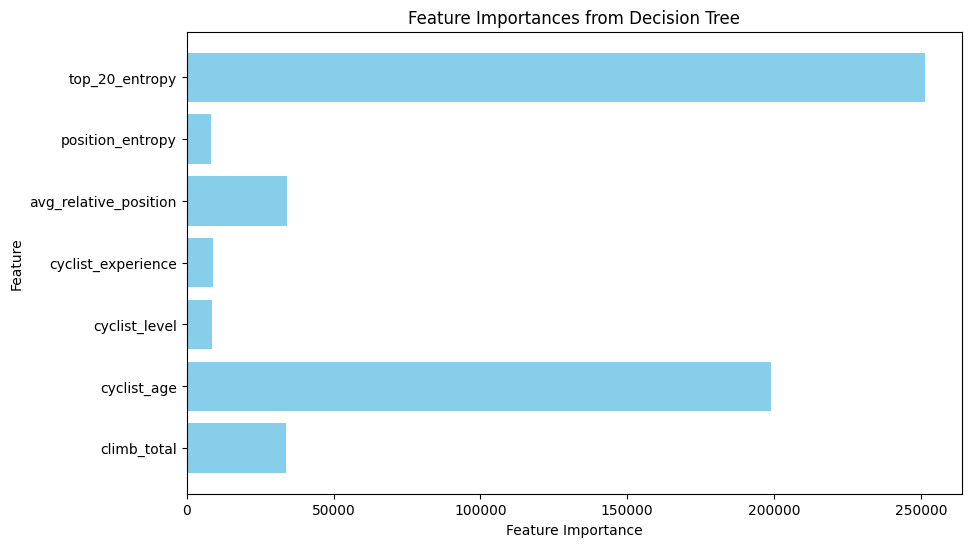
\includegraphics[width=0.4\linewidth]{images/CLASSIFICATION/gmb_feat_import.png}
    \caption{\small Feature importance plot for the GBM Model}
    \label{fig:gbm-feat-importance}
\end{figure}

\section{XAI}
To address explainability, following the professors' advice, we decided to apply the methods discussed in class to better understand the decisions made by the best model (GBM with SMOTETomek) in classifying the data.
More specifically, we compared the native explanation of the \enquote{LGBMClassifier} with the \enquote{SHAP} explanation, using both interventional and distributional approaches on a subset of the dataset, as well as locally on individual instances. We also applied \enquote{LIME} and \enquote{LORE} for local explanations on individual instances, with the latter used to generate counterfactual rules.

\subsection{SHAP explanations}

We used the SHAP TreeExplainer to generate SHAP values for the Gradient Boosting Machine, testing it on the first 400 instances of the test set for computational efficiency. Two explanation approaches were applied: the interventional explanation algorithm which perturbs features based on a causal model, and the distributional explanation algorithm which conditions the distribution learned from the training data.

The SHAP beeswarm plot in \autoref{fig:beeswarm} highlights the primary factors influencing the model's predictions, with key features including \textit{avg\_relative\_position}, \textit{climb\_total}, and \textit{position\_entropy}. Average relative position consistently shows a strong positive impact, particularly for low values, while climb total exhibits a diverse and variable influence across the dataset, with lower values influencing positively. Top 20 entropy similarly to average relative position influences negatively for higher values and positively for lower ones. On the other hand, features like \textit{cyclist\_experience} and \textit{cyclist\_level} have minimal impact, as their SHAP values remain near zero. 
The plot suggests that the model's decisions align with expected trends: cyclists with lower average positions or lower entropy in their results are more likely to maintain a spot in the top 20.

From the distributional perspective, \textit{cyclist\_age} consistently has a negative effect, while \textit{climb\_total} and \textit{position\_entropy} exhibit greater variability, with lower values contributing to higher positive SHAP values. \textit{top\_20\_entropy} has a negative contribution for lower values and a positive contribution for higher values, which appears to contradict expectations. Finally, we observe that the features predominantly drive predictions toward negative outcomes, with only a few contributing modestly toward positive labels.

While the visualizations effectively highlight the critical features and their contributions, they also expose overlapping distributions and low-impact features, pointing to potential redundancy. 

\begin{figure}[H]
    \centering
    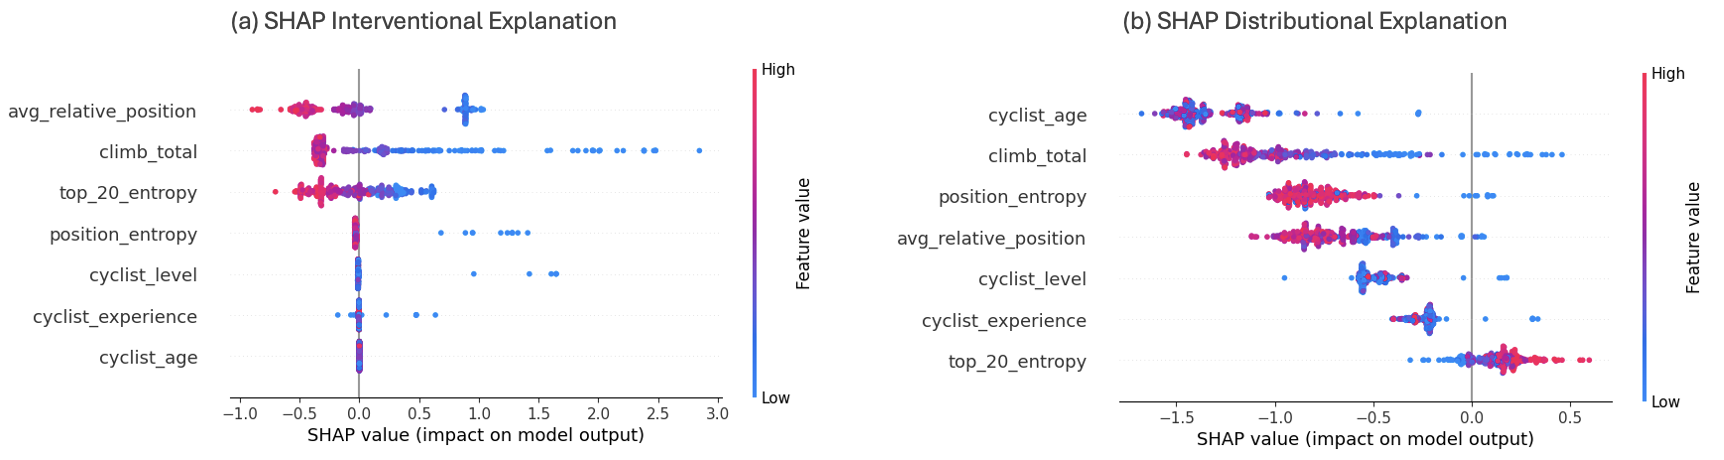
\includegraphics[width=0.9\linewidth]{images//XAI/beeswarm.png}
    \caption{\small SHAP beeswarm plot both for interventional and distributional approaches}
    \label{fig:beeswarm}
\end{figure}

\noindent In selecting features for the dependence plot, we prioritized the \textit{avg\_relative\_position} because it is one of the most important features for all methods. The feature found to be dependent is \textit{top\_20\_entropy}, another key feature. The plot in \autoref{fig:dependence_plot} shows the relationship between the two features in terms of SHAP values for the average relative position as the two vary.

The interventional explanation plot indicates that for \textit{average\_relative\_position} and \textit{top\_20\_entropy} values close to 0, the model predicts the highest SHAP value, suggesting a positive classification. This observation is reasonable, as low entropy and low average relative positions could indicate either a very strong cyclist or one with limited simpler race participation, where competing in simpler events often results in higher placements. As both entropy and average position increase, the SHAP value remains positive. This is because strong cyclists generally achieve good average placements but exhibit higher entropy due to strategic variations, as observed in \autoref{subsec:extra_analysis}. For intermediate values of the \textit{average\_relative\_position}, the SHAP value becomes insignificant both for higher or lower entropy.

For lower entropy values combined with higher average relative positions, the model tends to suggest a negative SHAP value. This is logical, as a cyclist with high average relative positions is unlikely to be very strong and its entropy is low because he typically places poorly.

\begin{figure}[H]
    \centering
    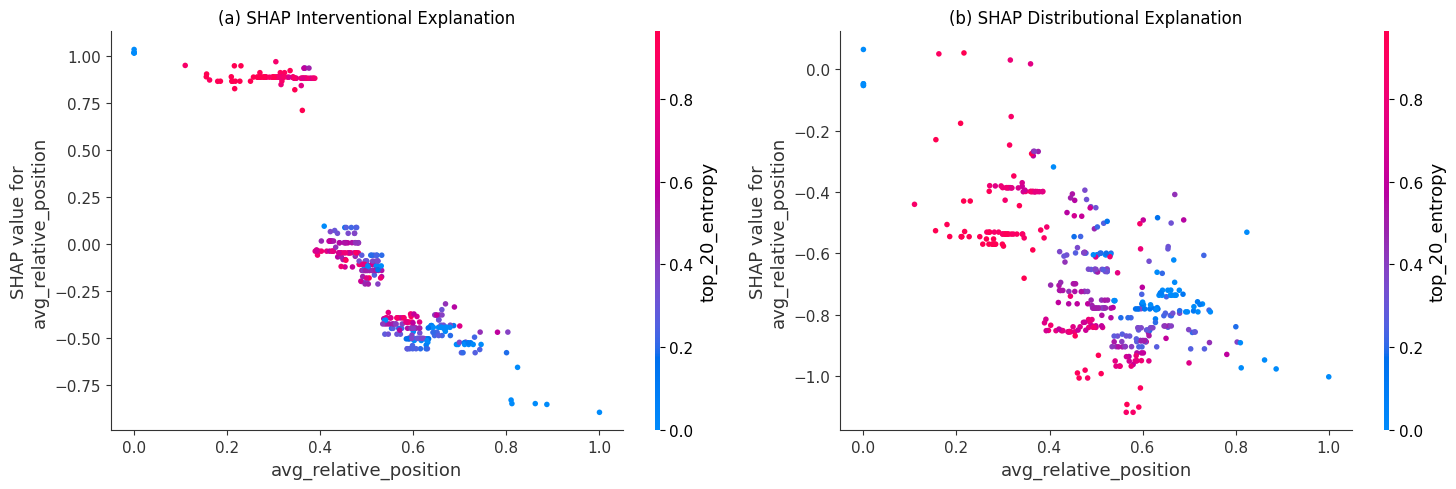
\includegraphics[width=0.9\linewidth]{images//XAI/dependence_plot.png}
    \caption{\small SHAP dependence plot both for interventional and distributional approaches}
    \label{fig:dependence_plot}
\end{figure}

The final SHAP analysis involves the difference in distributional and interventional approaches. The line plot in \autoref{fig:differences} (a) shows the distribution of maximum differences between interventional and distributional SHAP explanations for each instance. The peak around 1.4 indicates that most instances exhibit a maximum discrepancy of approximately 1.4, with a rapid drop in density beyond 1.6, suggesting large differences are rare. The narrow distribution indicates consistency, with only a few outliers showing significant differences. Overall, the two explanation methods generally agree, with limited divergence. 

The scatter plot in \autoref{fig:differences} (b) shows the maximum observed differences in SHAP values for each feature. Features like \textit{climb\_total} and \textit{cyclist\_age} exhibit the highest discrepancies, suggesting they may be more sensitive to the explanation method or involve complex interactions. In contrast, features such as \textit{top\_20\_entropy} and \textit{position\_entropy} show minimal differences, indicating stability across methods.

\begin{figure}[H]
    \centering
    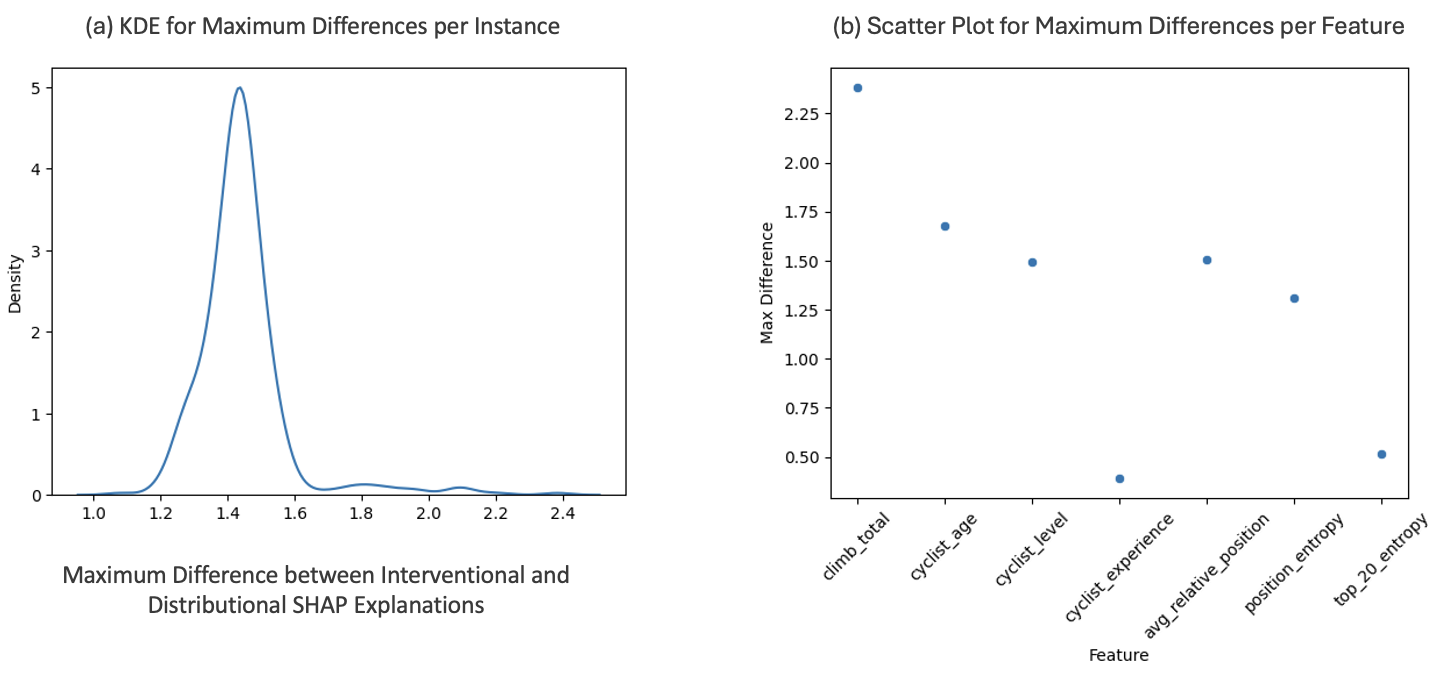
\includegraphics[width=0.8\linewidth]{images//XAI/differences.png}
    \vspace{-5pt}
    \caption{ \small SHAP explanation differences across instances (a) and features (b)}
    \label{fig:differences}
\end{figure}


\subsection{LORE local explanations and Counterfactual}
Regarding the LORE explanation, we focused on providing local explanations for individual data points, extracting rules, and counterfactuals, and assessing fidelity. Our focus is on understanding the conditions under which class 1 is predicted, given the models' low performance in this class.

In \autoref{fig:lore_tp} we observe the extracted rule (a) and most relevant counterfactuals (b) for random true positive data.
This rule indicates that the model heavily relies on the top 20 entropy and average relative position features. Specifically, the rule suggests that higher entropy combined with a lower average relative position is indicative of a strong cyclist. This may imply that cyclists with high entropy are highly experienced, while a low average relative position reflects consistently strong placements overall.
The high fidelity of 99.5\% reinforces the reliability of these observations.

\begin{figure}[H]
    \centering
    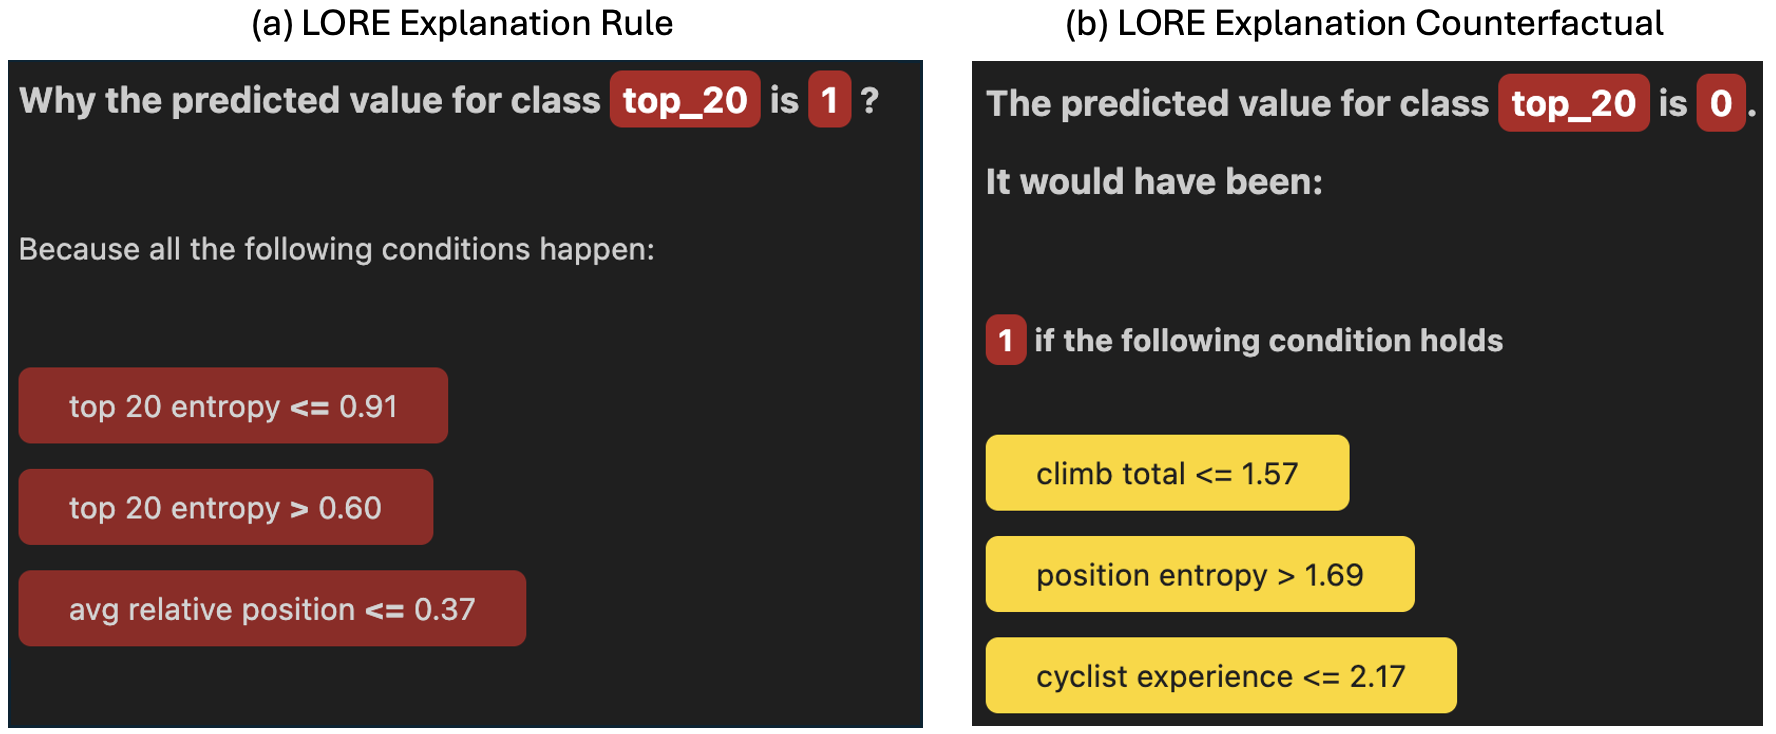
\includegraphics[width=0.7\linewidth]{images//XAI/lore_tp.png}
    \vspace{-5pt}
    \caption{ \small{LORE Rule (a) and Counterfactual (b) on True Positive Data}}
    \label{fig:lore_tp}
\end{figure}

\noindent \autoref{fig:lore_fn} shows the extracted rule (a) and most relevant counterfactuals (b) for a random false positive negative.

Low values of top 20 entropy and position entropy suggest the cyclist might be inexperienced, as consistent placements are unlikely to all be good. This may reflect a strategic focus on specific races or limited exposure to diverse scenarios, unlike experienced cyclists who show more varied results across conditions as seen also in the extra analysis. In fact, as counterfactuals, the model suggests a higher entropy and a low average relative position, indicating a good position until that race. The top 20 entropy value in this rule is not useful, as the maximum for this feature is 1.
Also in this case fidelity is very high (98.5\%), reinforcing the reliability of extracted rules.

\begin{figure}[H]
    \centering
    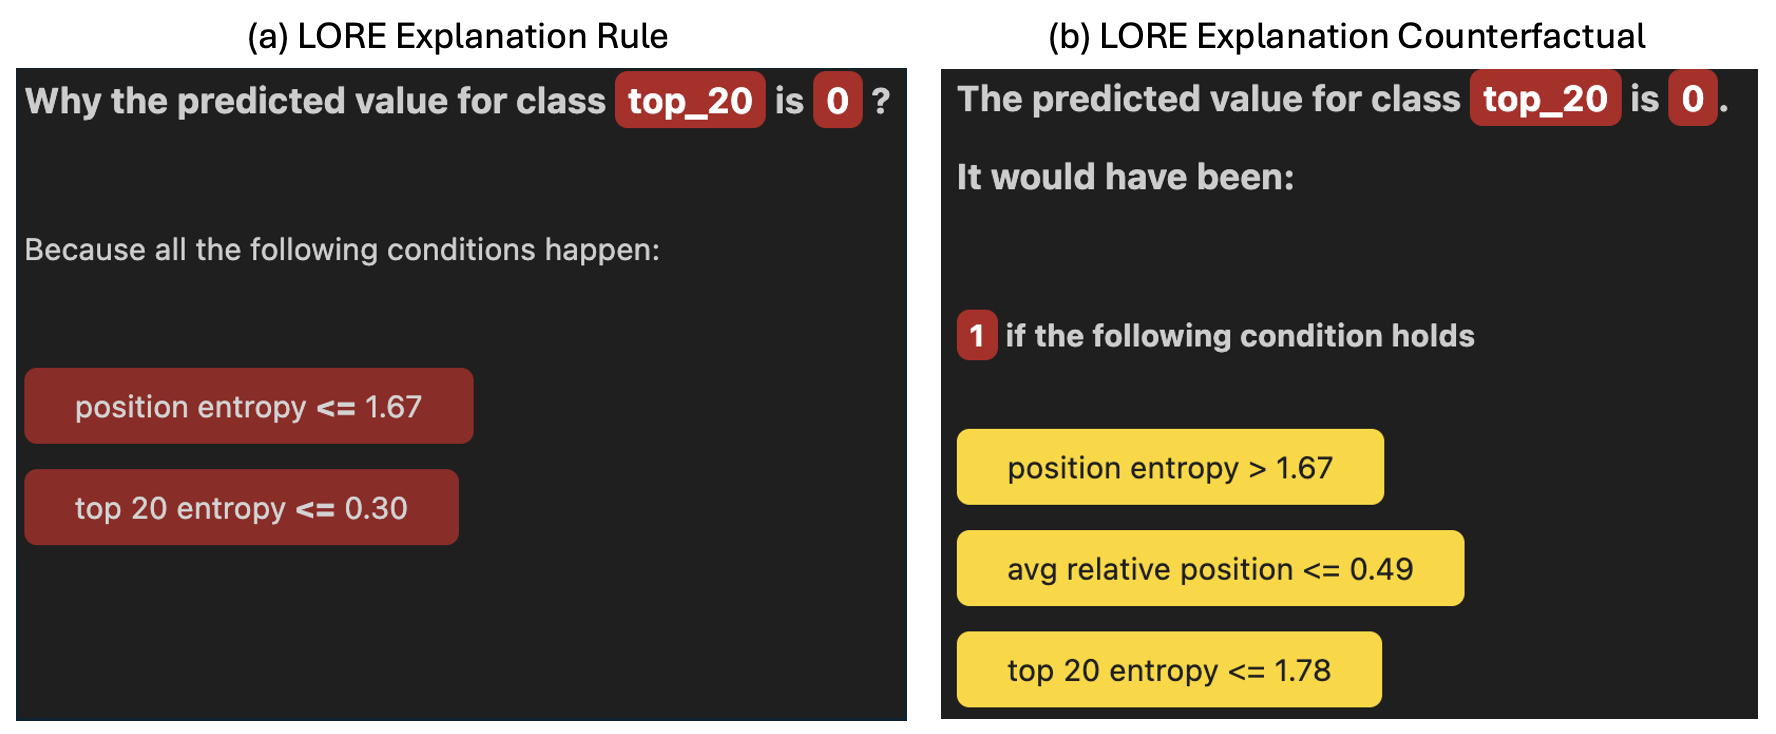
\includegraphics[width=0.7\linewidth]{images//XAI/lore_fn.png}
    \caption{ \small{LORE Rule (a) and Counterfactual (b) on False Negative Data}}
    \label{fig:lore_fn}
\end{figure}

\noindent Explanation rules and counterfactuals for true negative and false positive can be found in the notebook.

\subsection{LIME}

\noindent
\textbf{Analysis of the Impact of Feature Corruption on F1 Score}\\
This analysis identifies the features that have the greatest impact on model performance in noisy conditions and highlights those that are most resilient. The LIME results show that the features \textit{climb\_total}, \textit{avg\_relative\_position}, and \textit{top\_20\_entropy} exhibit high sensitivity to noise, with consistent performance drops around $-0.60$ to $-0.62$ in weighted f1. This suggests that these features are not only crucial to the model's predictions but also highly sensitive to variability, potentially making the model vulnerable to inaccuracies when these inputs deviate from expected values. In contrast, \textit{cyclist\_age} shows better robustness, with smaller performance drops around $-0.51$ and some improvement at certain noise levels. 

The overall trend of relatively stable performance across increasing noise magnitudes highlights the resilience of the model to moderate perturbations. However, the consistent negative differences, especially for key features, reveal a potential over-reliance. This dependency could undermine the model's generalization ability in real-world scenarios where data variability is inevitable.\\

\noindent
\textbf{Local Analysis of predictions}\\
In \autoref{fig:lime} (a) test \textit{top\_20\_entropy} turns out to be the most influential feature, contributing negatively to the predicted value and indicating that an increase in it significantly reduces the model result. \textit{avg\_relative\_position} has a moderate positive impact contributing to an increase in the predicted value although with less weight than \textit{top\_20\_entropy}. As for the other features, almost minimal contributions are observed, some positive and some negative. \\
In \autoref{fig:lime}, for a false negative data, the features \textit{top\_20\_entropy} and \textit{avg\_relative\_position} still turn out to be the most influential for prediction. Unlike the previous case \textit{top\_20\_entropy} contributes positively. Another difference is that while in the previous case, \textit{top\_20\_entropy} had a much greater weight than \textit{avg\_relative\_position} in this example their values turn out to be more similar. As in example 1, the other features show much less contribution although slightly more, some positive some negative but still close to zero.

\begin{figure}[H]
    \centering
    \includegraphics[width=1\linewidth]{images//XAI/LIME.png}
    \caption{\small LIME local analysis on true positive data (a) and false negative data (b)}
    \label{fig:lime}
\end{figure}

Similar to the findings from other explainability methods, LIME also identifies \textit{top\_20\_entropy} and \textit{avg\_relative\_position} as the most relevant features, with \textit{top\_20\_entropy} being the dominant factor in the true positive case and \textit{avg\_relative\_position} playing a key role in the false negative case.

\end{document}
